\documentclass[a4paper, 12pt, titlepage]{report}
\usepackage{graphicx}
\usepackage{fullpage}
\usepackage{float}
\usepackage{longtable}
\usepackage{amsmath}
\usepackage[normalem]{ulem}
\usepackage{booktabs}
\usepackage{array}
\usepackage{tikz}
\usepackage{booktabs}
\newcommand{\tabitem}{~~\llap{\textbullet}~~}
\setlength{\tabcolsep}{18pt}
\renewcommand{\arraystretch}{1.5}
\renewcommand{\chaptername}{Study Unit}
\begin{document}
\linespread{1.5}
\title{CMPG311 - Databases}
\author{Compiled by Affaan Muhammad}
\date{Semester 1 2020}
\maketitle
\tableofcontents{}
\chapter{Database Systems and Data Models}
Outcomes:
\begin{itemize}
\item Define the most important concepts relating to databases;
\item Define Big Data concepts;
\item Describe how databases have developed;
\item Evaluate the functioning of file systems and discuss the differences between database systems and file systems;
\item Describe the basic building blocks of data modelling; and
\item Discuss and classify database models.
\end{itemize}
\section{Why Databases?}
In today’s world, data is ubiquitous (abundant, global, everywhere) and pervasive (unescapable, prevalent, persistent). Data is not only ubiquitous and pervasive; it is also essential for organizations to survive and prosper.

\section{Data versus Information}
\textbf{Data} consists of raw facts. The word raw indicates that the facts have not yet been processed to reveal their meaning.
\textbf{Information} is the result of processing raw data to reveal its meaning. Data processing can be as simple as organizing data to reveal patterns or as complex as making forecasts or drawing inferences using statistical modeling. To reveal meaning, information requires context. Keep in mind that raw data must be properly \emph{formatted} for storage, processing, and presentation.
In this “information age,” production of accurate, relevant, and timely information is the key to good decision making. In turn, good decision making is the key to business survival in a global market. We are now said to be entering the “knowledge age.”
Data is the foundation of information, which is the bedrock of knowledge - that is, the body of information and facts about a specific subject. Knowledge implies familiarity, awareness, and understanding of information as it applies to an environment. A key characteristic of knowledge is that “new” knowledge can be derived from “old” knowledge.
\\ \\ Key points:
\begin{itemize}
\item Data constitutes the building blocks of information.
\item Information is produced by processing data.
\item Information is used to reveal the meaning of data.
\item Accurate, relevant, and timely information is the key to good decision making.
\item Good decision making is the key to organizational survival in a global environment.
\end{itemize}
\textbf{Data management} is a discipline that focuses on the proper generation, storage, and retrieval of data. Given the crucial role that data plays, it should not surprise you that data management is a core activity for any business, government agency, service organization, or charity.

\section{Introducing the Database}
A \textbf{database} is a shared, integrated computer structure that stores a collection of the following:
\begin{itemize}
\item End-user data—that is, raw facts of interest to the end user
\item \textbf{Metadata}, or data about data, through which the end-user data is integrated and managed
\end{itemize}
The metadata describes the data characteristics and the set of relationships that links the data found within the database. For example, the metadata component stores information such as the name of each data element, the type of values (numeric, dates, or text) stored on each data element, and whether the data element can be left empty. The metadata provides information that complements and expands the value and use of the data. In short, metadata presents a more complete picture of the data in the database. Given the characteristics of metadata, you might hear a database described as a “collection of \emph{self-describing} data.”\\
A \textbf{DataBase Management System (DBMS)} is a collection of programs that manages the database structure and controls access to the data stored in the database.
\subsection{Role and Advantages of the DBMS}
The DBMS serves as the intermediary between the user and the database. The database structure itself is stored as a collection of files, and the only way to access the data in those files is through the DBMS. The DBMS receives all application requests and translates them into the complex operations required to fulfill those requests. The DBMS hides much of the database’s internal complexity from the application programs and users.
\noindent In particular, a DBMS provides these advantages:
\begin{itemize}
\item \emph{Improved data sharing} - The DBMS helps create an environment in which end users have better access to more and better-managed data.
\item \emph{Improved data security} - The more users access the data, the greater the risks of data security breaches. Corporations invest considerable amounts of time, effort, and money to ensure that corporate data is used properly. A DBMS provides a framework for better enforcement of data privacy and security policies.
\item \emph{Better data integration} - Wider access to well-managed data promotes an integrated view of the organization’s operations and a clearer view of the big picture. It becomes much easier to see how actions in one segment of the company affect other segments.
\item \emph{Minimized data inconsistency} - \textbf{Data inconsistency} exists when different versions of the same data appear in different places.
\item \emph{Improved data access} - The DBMS makes it possible to produce quick answers to ad hoc queries. From a database perspective, a \textbf{query} is a specific request issued to the DBMS for data manipulation—for example, to read or update the data. Simply put, a query is a question, and an \textbf{ad hoc query} is a spur-of-the-moment question. The
DBMS sends back an answer (called the \textbf{query result set}) to the application. For example, when dealing with large amounts of sales data, end users might want quick answers to questions (ad hoc queries).
\item \emph{Improved decision making} - Better-managed data and improved data access make it possible to generate better-quality information, on which better decisions are based. The quality of the information generated depends on the quality of the underlying data. \textbf{Data quality} is a comprehensive approach to promoting the accuracy, validity, and timeliness of the data. While the DBMS does not guarantee data quality, it provides a framework to facilitate data quality initiatives.
\item \emph{Increased end-user productivity} - The availability of data, combined with the tools that transform data into usable information, empowers end users to make quick, informed decisions that can make the difference between success and failure in the global economy.
\end{itemize}

\subsection{Types of Databases}
A DBMS can be used to build many different types of databases. Each database stores a
particular collection of data and is used for a specific purpose. Over the years, as technology and innovative uses of databases have evolved, different methods have been used
to classify databases. For example, databases can be classified by the number of users
supported, where the data is located, the type of data stored, the intended data usage,
and the degree to which the data is structured.
Definitions to note:
\begin{itemize}
\item \textbf{Single-user Database} - A database that supports only one user at a time.
\item \textbf{Desktop Database} - A single-user database that runs on a personal computer.
\item \textbf{Multiuser Database} - A database that supports multiple concurrent users.
\item \textbf{Workgroup Database} - A multiuser database that usually supports fewer than 50 users or is used for a specific department in an organization.
\item \textbf{Enterprise Database} - The overall company data representation, which provides support for present and expected future needs.
\item \textbf{Centralized Database} - A database located at a single site.
\item \textbf{Distributed Database} - A logically related database that is stored in two or more physically independent sites.
\item \textbf{Cloud Database} - A database that is created and maintained using cloud services, such as Microsoft Azure or Amazon AWS.
\item \textbf{General-purpose Database} - A database that contains a wide variety of data used in multiple disciplines.
\item \textbf{Discipline-specific Database} - A database that contains data focused on specific subject areas.
\item \textbf{Operational Database} - A database designed primarily to support a company’s day-to-day operations. Also known as a \emph{transactional database, OLTP database, or production database}.
\item \textbf{Online Transaction Processing (OLTP) Database} - \emph{See operational database}.
\item \textbf{Transactional Database} - \emph{See operational database}.
\item \textbf{Production Database} - \emph{See operational database}. 
\item \textbf{Analytical Database} - A database focused primarily on storing historical data and business metrics used for tactical or strategic decision making. 
\item \textbf{Data Warehouse} - A specialized database that stores historical and aggregated data in a format optimized for decision support. 
\item \textbf{Online Analytical Processing (OLAP)} - A set of tools that provide advanced data analysis for retrieving, processing, and modeling data from the data warehouse. 
\item \textbf{Business Intelligence} - A set of tools and processes used to capture, collect, integrate, store, and analyze data to support business decision making. 
\item \textbf{Unstructured Data} - Data that exists in its original, raw state; that is, in the format in which it was collected. 
\item \textbf{Structured Data} - Data that has been formatted to facilitate storage, use, and information generation. 
\item \textbf{Semistructured Data} - Data that has already been processed to some extent.
\item \textbf{Extensible Markup Language (XML)} - A metalanguage used to represent and manipulate data elements. Unlike other markup languages, XML permits the manipulation of a
document’s data elements.
\item \textbf{XML Database} - Supports the storage and management of semistructured XML data.
\item \textbf{Social Media} - Web and mobile technologies that enable “anywhere, anytime, always on” human interactions.
\item \textbf{NoSQL} - A new generation of DBMS that is not based on the traditional relational database model.
\end{itemize}
\section{Why Database Design is Important}
\textbf{Database design} refers to the activities that focus on the design of the database
structure that will be used to store and manage end-user data. The process yields the description of the database structure and determines the database components. It is the second phase of the database life cycle.\\
Proper database design requires the designer to identify precisely the database’s expected use. Designing a transactional database emphasizes accurate and consistent data and operational speed. Designing a data warehouse database emphasizes the use of historical and aggregated data. Designing a database to be used in a centralized, single-user environment requires a different approach from that used in the design of a distributed, multiuser database. 

\section{Evolution of File System Data Processing}
\subsection{Manual File Systems}
Historically, such systems were often manual, paper-and-pencil systems. The papers within these systems were organized to facilitate the expected use of the data. Typically, this was accomplished through a system of file folders and filing cabinets.
However, as organizations grew and as reporting requirements became more complex, keeping track of data in a manual file system became more difficult. Therefore, companies looked to computer technology for help.

\subsection{Computerized File Systems}
Terminology developed around databases:
\begin{itemize}
\item \textbf{Data Processing (DP) Specialist} - The person responsible for developing and managing a computerized file processing system.
\item \textbf{Data} - Raw facts.
\item \textbf{Field} - A character or group of characters (alphabetic or numeric) that has a specific meaning. A field is used to define and store data.
\item \textbf{Record} - A logically connected set of one or more fields that describes a person, place, or thing.
\item \textbf{File} - A collection of related records.
\end{itemize}

\subsection{Modern End-User Productivity Tools}
Personal computer spreadsheet programs such as Microsoft Excel are widely used by business users, and they allow the user to enter data in a series of rows and columns so the data can be manipulated using a wide range of functions. The popularity of spreadsheet applications has enabled users to conduct sophisticated data analysis that has greatly enhanced their ability to understand the data and make better decisions. However, a common misuse of spreadsheets is as a substitute for a database.
\section{File System Data Processing Problems}
The following problems are noted:
\begin{itemize}
\item \emph{Lengthy development times}
\item \emph{Difficulty of getting quick answers}
\item \emph{Complex system administration}
\item \emph{Lack of security and limited data sharing}
\item \emph{Extensive programming}
\end{itemize}

\subsection{Structural and Data Dependence}
\begin{itemize}
\item \textbf{Structural Dependence} - A data characteristic in which a change in the database schema affects data access, thus requiring changes in all access programs. 
\item \textbf{Structural Independence} - A data characteristic in which changes in the database schema do not affect data access.
\item \textbf{Data Type} - Defines the kind of values that can be used or stored. Also, used in programming languages and database systems to determine the operations that can be applied to such data.
\item \textbf{Data Dependence} - A data condition in which data representation and manipulation are dependent on the physical data storage characteristics.
\item \textbf{Data Independence} - A condition in which data access is unaffected by changes in the physical data storage characteristics. 
\item \textbf{Logical Data Format} - The way a person views data within the context of a problem domain.
\item \textbf{Physical Data Format} - The way a computer “sees” (stores) data.
\end{itemize}

\subsection{Data redundancy}
\begin{itemize}
\item \textbf{Islands of Information} - In the old file system environment, pools of independent, often duplicated, and inconsistent data created and managed by different departments.
\item \textbf{Data Integrity} - In a relational database, a condition in which the data in the database complies with all entity and referential integrity constraints. Also defined as the condition in which all of the data in the database is consistent with the real-world events and conditions. In other words, data integrity means the following:
\begin{itemize}
\item \emph{Data is accurate} — there are no data inconsistencies.
\item \emph{Data is verifiable} — the data will always yield consistent results.
\end{itemize}
\item \textbf{Data Redundancy} - Exists when the same data is stored unnecessarily at different places. This Uncontrolled data redundancy sets the stage for the following:
\begin{itemize}
\item \emph{Poor data security} - Having multiple copies of data increases the chances for a copy of
the data to be susceptible to unauthorized access.
\item \emph{Data inconsistency} - Data inconsistency exists when different and conflicting versions of the same data appear in different places.
\item \emph{Data-entry errors} Data-entry errors are more likely to occur when complex entries are made in several different files or recur frequently in one or more files.
\item \emph{Data integrity problems}
\end{itemize}
\end{itemize}

\subsection{Data Anomalies}
A \textbf{data anomaly} develops when not all of the required changes in the redundant data are made successfully. The data anomalies are commonly defined as follows:
\begin{itemize}
\item \emph{Update anomalies}
\item \emph{Insertion anomalies}
\item \emph{Deletion anomalies}
\end{itemize}

\section{Database Systems}
\subsection{The Database System Environment}
The term \textbf{database system} refers to an organization of components that define and regulate the collection, storage, management, and use of data within a database environment. From a general management point of view, the database system is composed of the five major parts: Hardware, Software, People, Procedures, and Data.
\begin{itemize}
\item \textbf{Hardware} - Refers to all of the system’s physical devices, including computers, storage devices, printers, network devices, and other devices.
\item \textbf{Software} - Although the most readily identified software is the DBMS itself, three types of software are needed to make the database system function fully: operating
system software, DBMS software, and application programs and utilities.
\begin{itemize}
\item \emph{Operating system software} manages all hardware components and makes it possible for all other software to run on the computers. Examples of operating system software are Microsoft Windows, Linux, Mac OS, UNIX, and MVS.
\item \emph{DBMS software} manages the database within the database system. Some examples of DBMS software are Microsoft’s SQL Server, Oracle Corporation’s Oracle, Oracle’s MySQL, and IBM’s DB2.
\item \emph{Application programs and utility software} are used to access and manipulate data in the DBMS and to manage the computer environment in which data access and manipulation take place. Application programs are most commonly used to access data within the database to generate reports, tabulations, and other information to facilitate decision making. Utilities are the software tools used to help manage the database system’s computer components. For example, all of the major DBMS vendors now provide graphical user interfaces (GUIs) to help create database structures, control database access, and monitor database operations.
\end{itemize}
\item \textbf{People} - This component includes all users of the database system. Five types of users can be identified in a database system:
\begin{itemize}
\item \emph{System administrators} oversee the database system’s general operations.
\item \emph{Database administrators} manage the DBMS and ensure that the database is functioning properly.
\item \emph{Database designers} design the database structure. They are, in effect, the database architects.
\item \emph{System analysts and programmers} design and implement the application programs. They design and create the data-entry screens, reports, and procedures through which end users access and manipulate the database’s data.
\item \emph{End users} are the people who use the application programs to run the organization’s daily operations.
\end{itemize}
\item \textbf{Procedures} - Are the instructions and rules that govern the design and use of the database system.
\item \textbf{Data} - The word data covers the collection of facts stored in the database.
\end{itemize}
\subsection{DBMS Functions}
A DBMS performs several important functions that are explained as follows:
\begin{itemize}
\item \emph{Data dictionary management} - The DBMS stores definitions of the data elements and their relationships (metadata) in a data dictionary. In turn, all programs that access
the data in the database work through the DBMS. The DBMS uses the \textbf{data dictionary} to look up the required data component structures and relationships, thus
relieving you from having to code such complex relationships in each program. \textbf{Data dictionary} is a DBMS component that stores metadata—data about data. It contains data definitions as well as data characteristics and relationships and may also include data that is external to the DBMS.
\item \emph{Data storage management} - The DBMS creates and manages the complex structures required for data storage, thus relieving you from the difficult task of defining and programming the physical data characteristics. A modern DBMS provides storage not only for the data but also for related data-entry forms or screen definitions, report definitions, data validation rules, procedural code, structures to handle video and picture formats, and so on. Data storage management is also important for database performance tuning. \textbf{Performance tuning} relates to the activities that make the database perform more efficiently in terms of storage and access speed.
\item \emph{Data transformation and presentation} - The DBMS transforms entered data to conform to required data structures. The DBMS relieves you of the chore of distinguishing between the logical data format and the physical data format.
\item \emph{Security management} - The DBMS creates a security system that enforces user security and data privacy. Security rules determine which users can access the database, which data items each user can access, and which data operations the user can perform.
\item \emph{Multiuser access control} - To provide data integrity and data consistency, the DBMS uses sophisticated algorithms to ensure that multiple users can access the database
concurrently without compromising its integrity.
\item \emph{Backup and recovery management} - The DBMS provides backup and data recovery to ensure data safety and integrity. Current DBMS systems provide special utilities that allow the DBA to perform routine and special backup and restore procedures.
\item \emph{Data integrity management} - The DBMS promotes and enforces integrity rules, thus minimizing data redundancy and maximizing data consistency. The data relationships stored in the data dictionary are used to enforce data integrity.
\item \emph{Database access languages and application programming interfaces} - The DBMS provides data access through a query language. A \textbf{query language} is a nonprocedural language—one that lets the user specify what must be done without having to specify how. \textbf{Structured Query Language (SQL)} is the de facto query language and data access standard supported by the majority of DBMS vendors. The DBMS also provides application programming interfaces to procedural languages such as COBOL, C, Java, Visual Basic.NET, and C\#.
\item \emph{Database communication interfaces} - A current-generation DBMS accepts end-user requests via multiple, different network environments.
\end{itemize}
\subsection{Managing the Database System}
Although the database system yields considerable advantages over previous data management approaches, database systems do carry significant disadvantages:
\begin{itemize}
\item \emph{Increased costs} - Database systems require sophisticated hardware and software and highly skilled personnel and costs can be substantial. Training, licensing, and regulation compliance costs are often overlooked when database systems are implemented.
\item \emph{Management complexity} - Database systems interface with many different technologies and have a significant impact on a company’s resources and culture.
\item \emph{Maintaining currency} - To maximize the efficiency of the database system, you must keep your system current. Therefore, you must perform frequent updates and apply
the latest patches and security measures to all components.
\item \emph{Vendor dependence} - Given the heavy investment in technology and personnel training, companies might be reluctant to change database vendors.
\item \emph{Frequent upgrade/replacement cycles} - DBMS vendors frequently upgrade their products by adding new functionality. Such new features often come bundled in new upgrade versions of the software. Some of these versions require hardware upgrades.
\end{itemize}

\section{Data Modeling and Data Models}
\textbf{Data modeling}, the first step in designing a database, refers to the process of creating a specific data model for a determined problem domain. (A \emph{problem domain} is a clearly defined area within the real-world environment, with a well-defined scope and boundaries that will be systematically addressed.) A data model is a relatively
simple representation, usually graphical, of more complex real-world data structures. In general terms, a model is an abstraction of a more complex real-world object or event. A
model’s main function is to help you understand the complexities of the real-world environment. Data modeling is an iterative, progressive process. You start with a simple understanding of the problem domain, and as your understanding increases, so does the level of detail of the data model.

\section{The Importance of Data Models}
Data models can facilitate interaction among the designer, the applications programmer, and the end user. A well-developed data model can even foster improved understanding of the organization for which the database design is developed. In short, data models are a communication tool. When a good database blueprint is available, it does not matter that an applications programmer’s view of the data is different from that of the manager or the end user. Conversely, when a good database blueprint is not available, problems are likely to ensue. Keep in mind that a house blueprint is an abstraction; you cannot live in the blueprint. Similarly, the data model is an abstraction; you cannot draw the required data out of the data model. Just as you are not likely to build a good house without a blueprint, you are equally unlikely to create a good database without first creating an appropriate data model.

\section{Data Model Basic Building Blocks}
The basic building blocks of all data models are entities, attributes, relationships, and constraints:
\begin{itemize}
\item An \textbf{entity} is a person, place, thing, or event about which data will be collected and stored. An entity represents a particular type of object in the real world, which means an entity is “distinguishable”—that is, each entity occurrence is unique and distinct.
\item An \textbf{attribute} is a characteristic of an entity.
\item A \textbf{constraint} is a restriction placed on data, usually expressed in the form of rules.
\item A \textbf{relationship} describes an association among entities:
\begin{itemize}
\item \emph{one-to-many (1:M or 1..*) relationship} - Associations among 2 or more entities that are used by data models. In a 1:M relationship, 1 entity instance is associated with many instances of the related entity.
\item \emph{many-to-many (M:N or *..*) relationship} - Association among 2 or more entities in which 1 occurrence of an entity is associated with many occurrences of a related entity and one occurrence of the related entity is associated with many occurrences of the first entity.
\item \emph{one-to-one (1:1 or 1..1) relationship} - Associations among 2 or more entities that are used by data models. In a 1:1 relationship, 1 entity instance is associated with only 1 instance of the related entity.
\end{itemize}
\end{itemize}

\section{Business Rules}
From a database point of view, the collection of data becomes meaningful only when it reflects properly defined \emph{business rules}. A \textbf{business rule} is a brief, precise, and unambiguous description of a policy, procedure, or principle within a specific organization. They are derived from a detailed description of an organization’s operations help to create and enforce actions within that organization’s environment. Additionally:
\begin{itemize}
\item They must be rendered in writing and updated to reflect any change in the organization’s operational environment.
\item They are used to define entities, attributes, relationships, and constraints. 
\item To be effective, they must be easy to understand and widely disseminated to ensure that every person in the organization shares a common interpretation of the rules.
\item They describe, in simple language, the main and distinguishing characteristics of the data \emph{as viewed by the company}.
\end{itemize}

\subsection{Discovering Business Rules}
The main sources of business rules are company managers, policy makers, department managers, and written documentation such as a company’s procedures, standards, and operations manuals. A faster and more direct source of business rules is direct interviews with end users.
The process of identifying and documenting business rules is essential to database design for several reasons:
\begin{itemize}
\item It helps to standardize the company’s view of data.
\item It can be a communication tool between users and designers.
\item It allows the designer to understand the nature, role, and scope of the data.
\item It allows the designer to understand business processes.
\item It allows the designer to develop appropriate relationship participation rules and constraints and to create an accurate data model.
\end{itemize}
Please note that not all business rules can be modeled.

\subsection{Translating Business Rules into Data Model Components}
As a general rule, a noun in a business rule will translate into an entity in the model, and a verb (active or passive) that associates the nouns will translate into a relationship among the entities. To properly identify the type of relationship, you should consider that relationships are bidirectional; that is, they go both ways.

\subsection{Naming Conventions}
Entity names should be descriptive of the objects in the business environment and use terminology that is familiar to the users. An attribute name should also be descriptive of the data represented by that attribute. It is also a good practice to prefix the name of an attribute with the name or abbreviation of the entity in which it occurs.

\section{The Evolution of Data Models}
The quest for better data management has led to several models that attempt to resolve the previous model’s critical shortcomings and to provide solutions to ever-evolving data management needs. These models represent schools of thought as to what a database is, what it should do, the types of structures that it should employ, and the technology that would be used to implement these structures.
\subsection{Hierarchical and Network Models}
The \textbf{hierarchical model} was developed in the 1960s to manage large amounts of data for complex manufacturing projects. The model’s basic logical structure is represented by an upside-down tree. The hierarchical structure contains levels, or segments. A \textbf{segment} is the equivalent of a file system’s record type. The top record is the root segment. Each segment has a 1:M relationship to the segment directly below it.
The \textbf{network model} was created to represent complex data relationships more effectively than the hierarchical model, to improve database performance, and to impose a database standard. In the network model, the user perceives the network database as a
collection of records in 1:M relationships. However, the network model allows a record to have more than one parent. The definitions of standard database concepts that emerged with the network model are still used by modern data models:
\begin{itemize}
\item The \textbf{schema} is the conceptual organization of the entire database as viewed by the database administrator.
\item The \textbf{subschema} defines the portion of the database “seen” by the application programs that actually produce the desired information from the data within the database.
\item A \textbf{data manipulation language (DML)} defines the environment in which data can be managed and is used to work with the data in the database.
\item A schema \textbf{data definition language (DDL)} enables the database administrator to define the schema components such as database
structure, schema, and subschema.
\end{itemize}

\subsection{The Relational Model}
The \textbf{relational model} was introduced in 1970 by E. F. Codd of IBM. The relational model’s foundation is a mathematical concept known as a relation, you can think of a \textbf{relation} (sometimes called a \textbf{table}) as a two-dimensional structure composed of intersecting rows and columns. Each row in a relation is called a \textbf{tuple}. Each column represents an attribute. The relational data model is implemented through a very sophisticated \textbf{relational database management system (RDBMS)}. The RDBMS performs the same basic functions provided by the hierarchical and network DBMS systems, in addition to a host of other functions that make the relational data model easier to understand and implement. Arguably the most important advantage of the RDBMS is its ability to hide the complexities of the relational model from the user. The RDBMS manages all of the physical details, while the user sees the relational database as a collection of tables in which data is stored. The user can manipulate and query the data in a way that seems intuitive and logical. Tables are related to each other through the sharing of a common attribute (a value in a column).
The relational model provides a minimum level of controlled redundancy to eliminate most of the redundancies commonly found in file systems.
The relationship type (1:1, 1:M, or M:N) is often shown in a relational schema. A \textbf{relational diagram} is a representation of the relational database’s entities, the attributes within those entities, and the relationships between those entities.
A relational table stores a collection of related entities. In this respect, the relational database table resembles a file, but there is a crucial difference between a table and a file: a table yields complete data and structural independence because it is a purely logical structure. How the data is physically stored in the database is of no concern to the user or the designer; the perception is what counts.
Another reason for the relational data model’s rise to dominance is its powerful and flexible query language. Most relational database software uses Structured Query Language (SQL), which allows the user to specify what must be done without specifying how. The RDBMS uses SQL to translate user queries into instructions for retrieving the requested data. SQL makes it possible to retrieve data with far less effort than any other database or file environment.
From an end-user perspective, any SQL-based relational database application involves three parts: a user interface, a set of tables stored in the database, and the SQL “engine.” Each of these parts is explained as follows:
\begin{itemize}
\item \emph{The end-user interface}. Basically, the interface allows the end user to interact with the data.
\item \emph{A collection of tables stored in the database}. In a relational database, all data is perceived to be stored in tables. The tables simply “present” the data to the end user in a way that is easy to understand. Each table is independent. Rows in different tables are related by common values in common attributes.
\item \emph{SQL engine}. Largely hidden from the end user, the SQL engine executes all queries, or data requests. Keep in mind that the SQL engine is part of the DBMS software. The end user uses SQL to create table structures and to perform data access and table maintenance. The SQL engine processes all user requests. Hence, SQL is said to be a declarative language that tells what must be done but not how.
\end{itemize}

\subsection{The Entity Relationship Model}
The conceptual simplicity of relational database technology triggered the demand for RDBMSs. In turn, the rapidly increasing requirements for transaction and information created the need for more complex database implementation structures, thus creating the need for more effective database design tools. Thus, the \textbf{entity relationship (ER) model}, or \textbf{ERM}, has become a widely accepted standard for data modeling. Peter Chen first introduced the ER data model in 1976; the graphical representation of entities and their relationships in a database structure quickly became popular because it complemented the relational data model concepts. The relational data model
and ERM combined to provide the foundation for tightly structured database design. ER models are normally represented in an entity relationship diagram (ERD), which uses graphical representations to model database components. You will learn how to use ERDs to design databases in Chapter 4, Entity Relationship (ER) Modeling. The ER model is based on the following components:
\begin{itemize}
\item \emph{Entity}. An entity is defined as anything about which data will be collected and stored. An entity is represented in the ERD by a rectangle, also known as an entity box. The name of the entity, a noun, is written in the center of
the rectangle. The entity name is generally written in capital letters and in singular form. Usually, when applying the ERD to the relational model, an entity is mapped to a relational table. Each row in the relational table is known as an \textbf{entity instance} or \textbf{entity occurrence} in the ER model. A collection of like entities is known as an \textbf{entity set}.
\item Each entity consists of a set of \emph{attributes} that describes particular characteristics of the entity.
\item \emph{Relationships}. They describe associations among data. Most relationships describe associations between two entities. When the basic data model components were introduced, three types of data relationships were illustrated: one-to-many (1:M), many-to-many (M:N), and one-to-one (1:1). The ER model uses the term connectivity to label the relationship types. The name of the relationship is usually an active or passive verb. The different types of ER notations are: the original \textbf{Chen notation}, the \textbf{Crow’s Foot notation}, and the newer \textbf{class diagram notation}, which is part of the Unified Modeling Language (UML).
\end{itemize}
\begin{figure}[H]
\centering
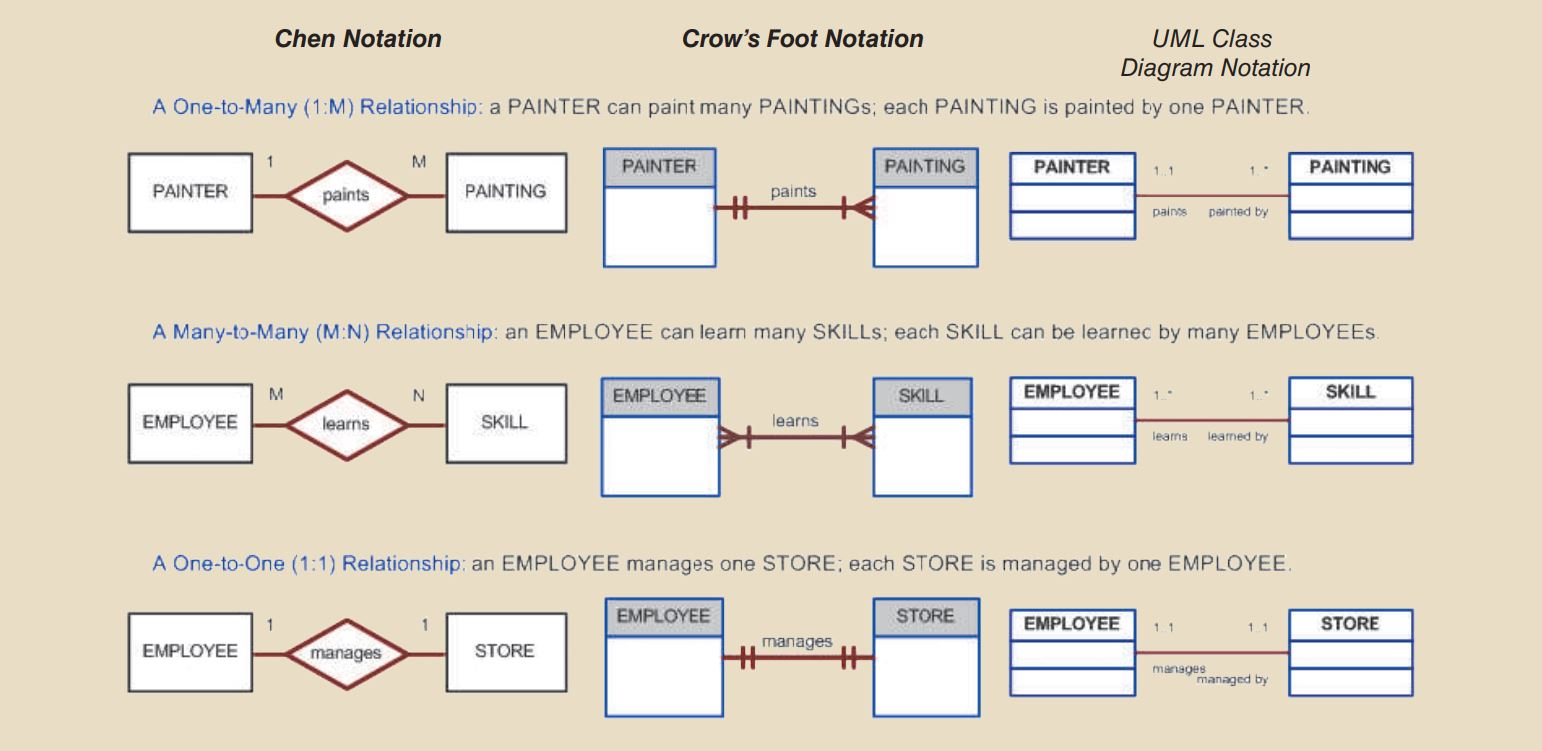
\includegraphics[scale=0.3]{ERNot}
\caption{The ER Model Notations}
\end{figure}
 
\subsection{The Object-Oriented Model}
Increasingly complex real-world problems demonstrated a need for a data model that more closely represented the real world. In the \textbf{object-oriented data model (OODM)}, both data and its relationships are contained in a single structure known as an \textbf{object}. In turn, the OODM is the basis for the \textbf{object-oriented database management system (OODBMs)}. An OODM reflects a very different way to define and use entities. Like the relational model’s entity, an object is described by its factual content. But, quite unlike an entity, an object includes information about relationships between the facts within the object, as well as information about its relationships with other objects. Therefore, the facts within the object are given greater \emph{meaning}. The OODM is said to be a \textbf{semantic data model} because \emph{semantic} indicates meaning.
The OO data model is based on the following components:
\begin{itemize}
\item An \textbf{object} is an abstraction of a real-world entity. More precisely, an object represents only one occurrence of an entity.
\item \textbf{Attributes} describe the properties of an object.
\item Objects that share similar characteristics are grouped in classes. A \textbf{class} is a collection of similar objects with shared structure (attributes) and behavior (methods). A class’s \textbf{method} represents a real-world action.
\item Classes are organized in a class hierarchy. The \textbf{class hierarchy} resembles an upsidedown tree in which each class has only one parent.
\item \textbf{Inheritance} is the ability of an object within the class hierarchy to inherit the attributes and methods of the classes above it.
\item Object-oriented data models are typically depicted using \textbf{Unified Modeling Language (UML)} class diagrams. UML is a language based on OO concepts that describes a set of diagrams and symbols you can use to graphically model a system. UML \textbf{class diagrams} are used to represent data and its relationships within the larger UML object-oriented system’s modeling language.
\end{itemize}
\subsection{Object/Relational and XML}
Facing the demand to support more complex data representations, the relational model’s main vendors evolved the model further and created the \textbf{extended relational data model (erDM)}. The ERDM adds many of the OO model’s features within the inherently simpler relational database structure. The ERDM gave birth to a new generation of relational databases that support OO features such as objects (encapsulated data and methods), extensible data types based on classes, and inheritance. That’s why a DBMS based on the ERDM is often described as an \textbf{object/relational database management system (O/r DBMs)}. Today, most relational database products can be classified as object/relational, and
they represent the dominant market share of OLTP and OLAP database applications. The success of the O/R DBMSs can be attributed to the model’s conceptual simplicity, data integrity, easy-to-use query language, high transaction performance, high availability, security, scalability, and expandability. In contrast, the OO DBMS is popular in niche markets such as computer-aided drawing/computer-aided manufacturing (CAD/
CAM), geographic information systems (GIS), telecommunications, and multimedia, which require support for more complex objects.
From the start, the OO and relational data models were developed in response to different problems. The OO data model was created to address very specific engineering needs, not the wide-ranging needs of general data management tasks. The relational
model was created with a focus on better data management based on a sound mathematical foundation. Given its focus on a smaller set of problem areas, it is not surprising that the OO market has not grown as rapidly as the relational data model market. The use of complex objects received a boost with the Internet revolution. When organizations integrated their business models with the Internet, they realized its potential to access, distribute, and exchange critical business information. This resulted in the widespread adoption of the Internet as a business communication tool. Within this environment, \textbf{extensible Markup Language (xML)} emerged as the defacto standard for the efficient and effective exchange of structured, semistructured, and unstructured data. Organizations that used XML data soon realized that they needed to manage large amounts of unstructured data such as word-processing documents, webpages, emails, and diagrams. To address this need, XML databases emerged to manage unstructured data within a native XML format. At the same time, O/R DBMSs added support for XML-based documents within their relational data structure.

\subsection{Emerging Data Models}
\textbf{Big Data} refers to a movement to find new and better ways to manage large amounts of web and sensor-generated data and derive business insight from it, while simultaneously providing high performance and scalability at a reasonable cost.
The term Big Data has been used in many different frameworks, from law to statistics to economics to computing. The basic characteristics of Big Data databases are:
\begin{itemize}
\item \emph{Volume} refers to the amounts of data being stored.
\item \emph{Velocity} refers not only to the speed with which data grows but also to the need to process this data quickly in order to generate information and insight.
\item \emph{Variety} refers to the fact that the data being collected comes in multiple different data formats. A great portion of these data comes in formats not suitable to be handled by the typical operational databases based on the relational model.
\end{itemize}
The problem is that the relational approach does not always match the needs of organizations with Big Data challenges:
\begin{itemize}
\item It is not always possible to fit unstructured, social media and sensor-generated data into the conventional relational structure of rows and columns.
\item Adding millions of rows of multiformat (structured and nonstructured) data on a daily basis will inevitably lead to the need for more storage, processing power, and sophisticated data analysis tools that may not be available in the relational environment.
\item Data analysis based on OLAP tools has proven to be very successful in relational environments with highly structured data. However, mining for usable data in the vast amounts of unstructured data collected from web sources requires a different approach.
\end{itemize}
Some of the most frequently used Big Data technologies are:
\begin{itemize}
\item \textbf{Hadoop} is a Java-based, open-source, high-speed, fault-tolerant distributed storage and computational framework. Hadoop uses low-cost hardware to create clusters of thousands of computer nodes to store and process data. Hadoop has several modules, but the two main components are Hadoop Distributed File System (HDFS) and MapReduce.
\begin{itemize}
\item \emph{Hadoop Distributed File system (HDFs)} is a highly distributed, fault-tolerant file storage system designed to manage large amounts of data at high speeds. In order to achieve high throughput, HDFS uses the write-once, read many model. This means that once the data is written, it cannot be modified. HDFS uses three types of nodes: a \textbf{name node} that stores all the metadata about the file system, a \textbf{data node} that stores fixed-size data blocks (that could be replicated to other data nodes), and a \textbf{client node} that acts as the interface between the user application and the HDFS.
\item \emph{Mapreduce} is an open-source application programming interface (API) that provides fast data analytics services. MapReduce distributes the processing of the data among thousands of nodes in parallel. MapReduce works with structured and nonstructured data. The MapReduce framework provides two main functions: Map and Reduce. In general terms, the Map function takes a job and divides it into smaller units of work, and the Reduce function collects all the output results generated from the nodes and integrates them into a single result set.
\end{itemize}
\item \textbf{NosQL} is a large-scale distributed database system that stores structured and unstructured data in efficient ways.
\end{itemize}
The new generation of databases have the following general characteristics:
\begin{itemize}
\item They are not based on the relational model and SQL; hence the name NoSQL.
\item They support highly distributed database architectures.
\item They provide high scalability, high availability, and fault tolerance.
\item They support very large amounts of sparse data (data with a large number of attributes but where the actual number of data instances is low).
\item They are geared toward performance rather than transaction consistency.
\end{itemize}

\section{Data Models - A Summary}
\begin{figure}[H]
\centering
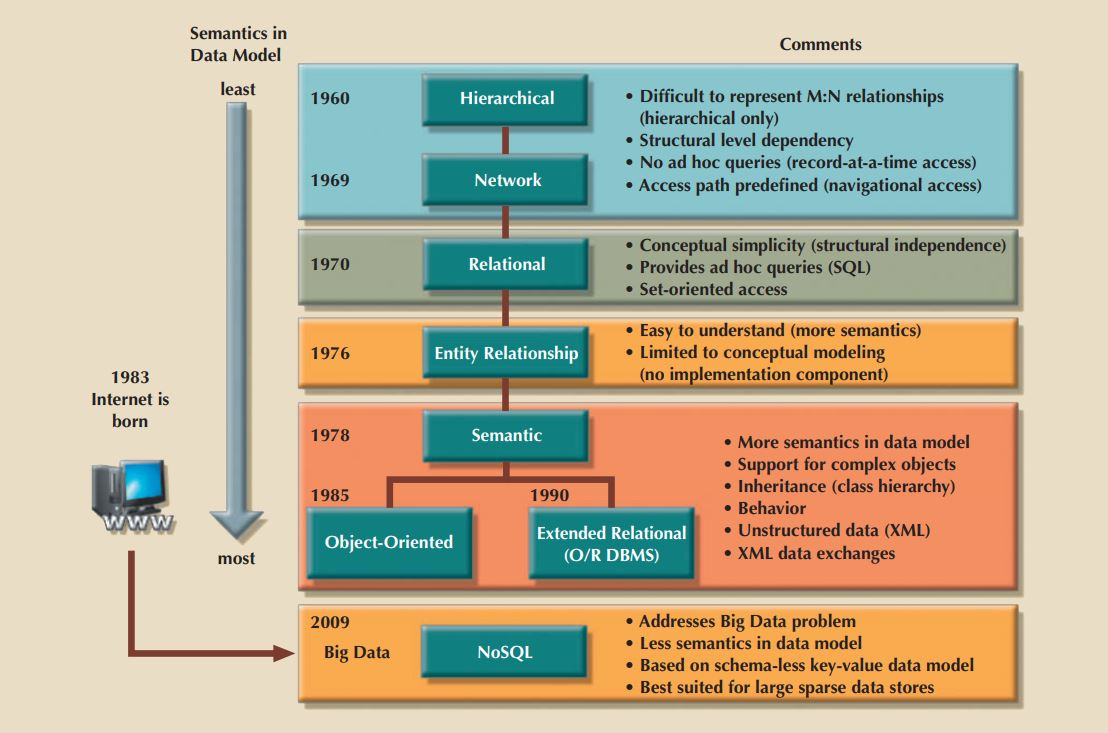
\includegraphics[scale=0.5]{DMSummary}
\caption{The Evolution of Data Models}
\end{figure}

\section{Degrees of Data Abstraction}
\begin{figure}[H]
\centering
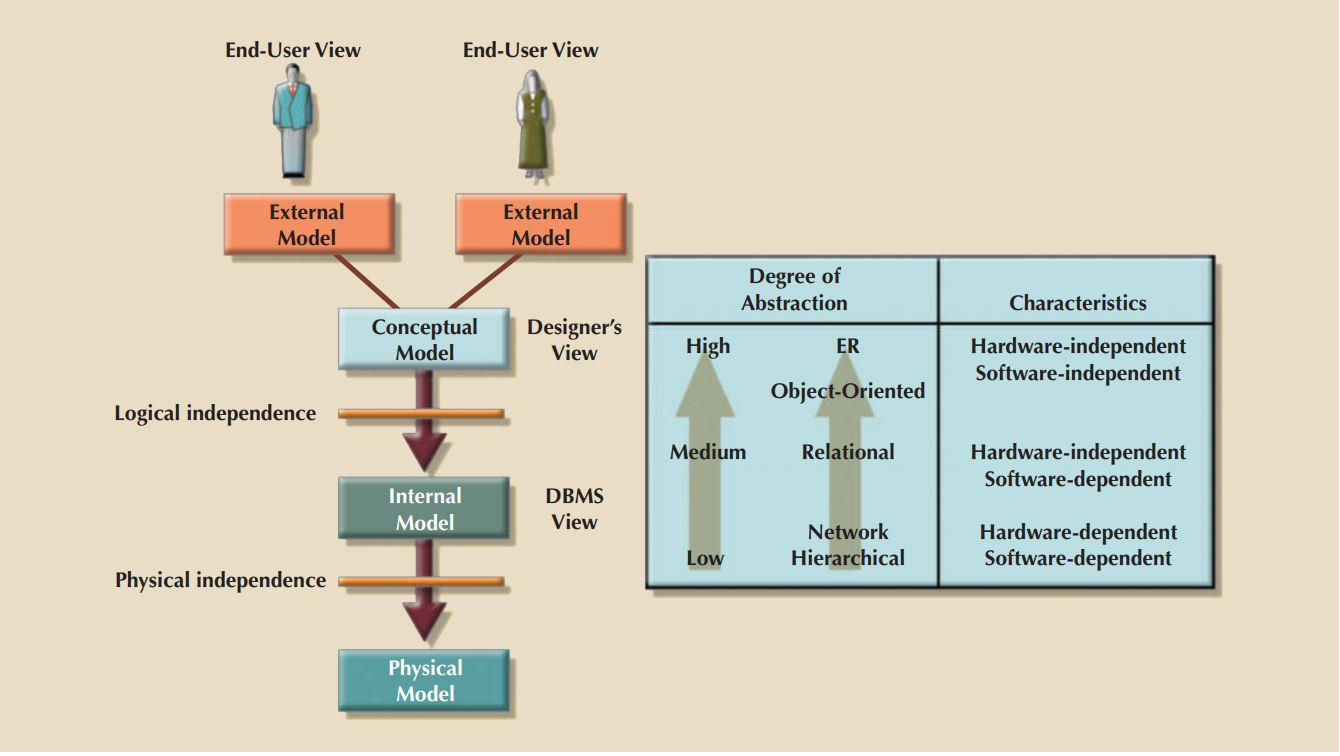
\includegraphics[scale=0.45]{DLAbs}
\caption{Data Abstraction Levels}
\end{figure}

\subsection{The External Model}
The \textbf{external model} is the end users’ view of the data environment. The term end users refers to people who use the application programs to manipulate the data and generate information. Companies are generally divided into several business units, such as sales, finance, and marketing. Each business unit is subject to specific constraints and requirements, and each one uses a subset of the overall data in the organization. Therefore, end users within those business units view their data subsets as separate from or external to other units within the organization. Because data is being modeled, ER diagrams will be used to represent the external views. A specific representation of an external view is known as an \textbf{external schema}. Also note that \emph{although the application views are isolated from each other, each view shares a common entity with the other view.}
The use of external views that represent subsets of the database has some important advantages:
\begin{itemize}
\item It is easy to identify specific data required to support each business unit’s operations.
\item It makes the designer’s job easy by providing feedback about the model’s adequacy.
\item It helps to ensure security constraints in the database design.
\item It makes application program development much simpler.
\end{itemize}

\subsection{The Conceptual Model}
The \textbf{conceptual model} represents a global view of the entire database by the entire organization. That is, the conceptual model integrates all external views (entities, relationships, constraints, and processes) into a single global view of the data in the enterprise. Also known as a \textbf{conceptual schema}, it is the basis for the identification and high-level description of the main data objects. The most widely used conceptual model is the ER model. The ERD is used to graphically \emph{represent} the conceptual schema. The conceptual model yields some important advantages:
\begin{itemize}
\item It provides a birdseye view of the data environment that is relatively easy to understand.
\item It is independent of both software and hardware. \textbf{Software independence} means that the model does not depend on the DBMS software used to implement the model. \textbf{Hardware independence} means that the model does not depend on the hardware used in the implementation of the model. Therefore, changes in either the hardware or the DBMS software will have no effect on the database design at the conceptual level. Generally, the term logical design refers to the task of creating a conceptual data model that could be implemented in any DBMS.
\end{itemize}

\subsection{The Internal Model}
Once a specific DBMS has been selected, the \textbf{internal model} maps the conceptual model to the DBMS. The internal model is the representation of the database as “seen” by the DBMS. An \textbf{internal schema} depicts a specific representation of an internal model, using the database constructs supported by the chosen database. Because the internal model depends on specific database software, it is said to be software dependent. Therefore, a change in the DBMS software requires that the internal model be changed to fit the characteristics and requirements of the implementation database model. When you can change the internal model without affecting the conceptual model, you have \textbf{logical independence}. However, the internal model is still hardware independent because it is unaffected by the type of computer on which the software is installed. Therefore, a change in storage devices or even a change in operating systems will not affect the internal model.

\subsection{The Physical Model}
The \textbf{physical model} operates at the lowest level of abstraction, describing the way data is saved on storage media such as magnetic, solid state, or optical media. The physical model requires the definition of both the physical storage devices and the (physical) access methods required to reach the data within those storage devices, making it both software and hardware dependent. The storage structures used are dependent on the software (the DBMS and the operating system) and on the type of storage devices the computer can handle. When you can change the physical model without affecting the internal model, you have \textbf{physical independence}. Therefore, a change in storage devices or methods and even a change in operating system will not affect the internal model.

\chapter{Database Design}
Outcomes:
\begin{itemize}
\item Discuss the primary aim of database design; and
\item Give an overview of the database design cycle.
\end{itemize}
\section{The Information System}
The database is part of a larger whole known as an \textbf{information system (IS)}, which provides for data collection, storage, transformation, and retrieval. The information system also helps transform data into information, and it allows for the management of both data and information. \textbf{Systems analysis} is the process that establishes the need for an information system and its extent. The process of creating an information system is known as \textbf{systems development}. The performance of an information system depends on three factors:
\begin{itemize}
\item Database design and implementation
\item Application design and implementation
\item Administrative procedures
\end{itemize}
In a broad sense, the term \textbf{database development} describes the process of database design and implementation.

\section{The Systems Development Life Cycle}
The \textbf{Systems Development Life Cycle (SDLC)} traces the history of an information system. The traditional SDLC is divided into five phases: planning, analysis, detailed systems design, implementation, and maintenance. The SDLC is an iterative process rather than a sequential process.

\subsection{Planning}
The SDLC planning phase yields a general overview of the company and its objectives. An initial assessment of the information flow-and-extent requirements must be made during this stage. Such an assessment should answer some important questions:
\begin{itemize}
\item \emph{Should the existing system be continued?}
\item \emph{Should the existing system be modified?}
\item \emph{Should the existing system be replaced?}
\end{itemize}
If a new system is necessary, the next question is whether it is feasible. The feasibility study must address the following:
\begin{itemize}
\item \emph{The technical aspects of hardware and software requirements}
\item \emph{The system cost}
\item \emph{The operational cost}
\end{itemize}

\subsection{Analysis}
Problems defined during the planning phase are examined in greater detail during the analysis phase. A macro analysis must be made both of individual needs and organizational needs, addressing questions such as:
\begin{itemize}
\item \emph{What are the requirements of the current system’s end users?}
\item \emph{Do those requirements fit into the overall information requirements?}
\end{itemize}
The analysis phase of the SDLC is, in effect, a thorough \emph{audit} of user requirements. The existing hardware and software systems are also studied during the analysis phase. The result of the analysis should be a better understanding of the system’s functional areas, actual and potential problems, and opportunities. End users and the system designers must work together to identify processes and uncover potential problem areas. Such cooperation is vital to defining the appropriate performance objectives by which the new system can be judged. The analysis phase also includes the creation of a logical systems design. When creating a logical design, the designer might use tools such as data flow diagrams (DFDs), hierarchical input process output (HIPO) diagrams, entity relationship (ER) diagrams, and even some application prototypes.

\subsection{Detailed Systems Design}
In the detailed systems design phase, the designer completes the design of the system’s processes. The design includes all the necessary technical specifications for the screens, menus, reports, and other devices that might help make the system a more efficient information generator. The steps are laid out for conversion from the old system to the new system.

\subsection{Implementation}
During the implementation phase, the hardware, DBMS software, and application programs are installed, and the database design is implemented. During the initial stages of the implementation phase, the system enters into a cycle of coding, testing, and debugging until it is ready to be delivered. The actual database is created, and the system is customized. The database contents might be loaded interactively or in batch mode. The system is subjected to exhaustive testing until it is ready for use. After testing is concluded, the final documentation is reviewed and printed and end users are trained. The system is in full operation at the end of this phase, but it will be continuously evaluated and fine-tuned.

\subsection{Maintenance}
Almost as soon as the system is operational, end users begin to request changes in it. Those changes generate system maintenance activities, which can be grouped into three types:
\begin{itemize}
\item \emph{Corrective maintenance} in response to systems errors
\item \emph{Adaptive maintenance} due to changes in the business environment
\item \emph{Perfective maintenance} to enhance the system
\end{itemize}

\section{The Database Life Cycle}
The \textbf{Database Life Cycle (DBLC)} contains six phases: database initial study, database design, implementation and loading, testing and evaluation, operation, and maintenance and evolution.
\subsection{The Database Initial Study}
The overall purpose of the database initial study is to:
\begin{enumerate}
\item \emph{Analyze the company situation}\\ The \emph{company situation} describes the general conditions in which a company operates, its organizational structure, and its mission. The following issues must be resolved:
\begin{enumerate}
\item \emph{What is the organization’s general operating environment, and what is its mission within that environment?} The design must satisfy the operational demands created by the organization’s mission.
\item \emph{What is the organization’s structure?} Knowing who controls what and who reports to whom is quite useful when you need to define required information flows, specific report and query formats, and so on.
\end{enumerate}
\item \emph{Define problems and constraints} \\
The process of defining problems might initially appear to be unstructured. Company end users often cannot precisely describe the larger scope of company operations or identify the real problems encountered during company operations. During the initial problem definition process, the designer is likely to collect very broad problem descriptions. After the initial declarations, the database designer must continue to probe carefully to generate additional information that will help define the problems within the larger framework of company operations. Finding precise answers is important, especially concerning the operational relationships among business units.
\item \emph{Define objectives} \\
A proposed database system must be designed to help solve at least the major problems identified during the problem discovery process. Note that the initial study phase also yields proposed problem solutions. The designer’s job is to make sure that his or her database system objectives correspond to those envisioned by the end users. In any case, the database designer must begin to address the following questions:
\begin{itemize}
\item What is the proposed system’s initial objective?
\item Will the system interface with other existing or future systems in the company?
\item Will the system share the data with other systems or users?
\end{itemize}
\item \emph{Define scope and boundaries} \\
The designer must recognize two sets of limits: scope and boundaries. The system’s \textbf{scope} defines the extent of the design according to operational requirements. Knowing the scope helps define the required data structures, the type and number of entities, the physical size of the database, and so on. The proposed system is also subject to limits known as \textbf{boundaries}, which are external to the system. These limits include budgets, personnel, and existing hardware and software.
\end{enumerate}

\subsection{Database Design}
This is arguably the most critical DBLC phase: making sure that the final product meets user and system requirements. You must concentrate on the data characteristics required to build the database model. There are two views of the data within the system: the business view of data as a source of information and the designer’s view of the data structure, its access, and the activities required to transform the data into information. Note that you can summarize the different views by looking at the terms what and how. Defining data is an integral part of the DBLC’s second phase.

\subsection{Implementation and Loading}
The output of the database design phase is a series of instructions detailing the creation of tables, attributes, domains, views, indexes, security constraints, and storage and performance guidelines. In this phase, you actually implement all these design specifications. Stages inclued:
\begin{enumerate}
\item Install the DBMS
\item Create the Database(s)
\item Load or Convert the Data
\end{enumerate}

\subsection{Testing and	Evaluation}
In the design phase, decisions were made to ensure integrity, security, performance, and recoverability of the database. During implementation and loading, these plans were put into place. In testing and evaluation, the DBA tests and fine-tunes the database to ensure that it performs as expected. Stages include:
\begin{enumerate}
\item Test the Database. \\ The following is normally tested:
\begin{itemize}
\item \emph{Physical security}
\item \emph{Password security }
\item \emph{Access rights}
\item \emph{Audit trails }
\item \emph{Data encryption}
\item \emph{Diskless workstations}
\end{itemize}
\item Fine-tune the Database
\item Evaluate the Database and Its Application Programs. \\ \\ Database backups can be performed at different levels:
\begin{itemize}
\item A \textbf{full backup}, or \emph{dump}, of the entire database. In this case, all database objects are backed up in their entirety.
\item A \textbf{differential backup} of the database, in which only the objects that have been updated or modified since the last full backup are backed up.
\item A \textbf{transaction log backup}, which backs up only the transaction log operations that are not reflected in a previous backup copy of the database. In this case, no other database objects are backed up. 
\end{itemize}
\end{enumerate}

\subsection{Operation}
Once the database has passed the evaluation stage, it is considered operational. At that point, the database, its management, its users, and its application programs constitute a
complete information system. The beginning of the operational phase invariably starts the process of system evolution. The demand for change is the designer’s constant concern, which leads to phase 6, maintenance and evolution.

\subsection{Maintenance and	Evolution}
The database administrator must be prepared to perform routine maintenance activities within the database. Some of the required periodic maintenance activities include:
\begin{itemize}
\item Preventive maintenance (backup)
\item Corrective maintenance (recovery)
\item Adaptive maintenance (enhancing performance, adding entities and attributes, and so on)
\item Assignment of access permissions and their maintenance for new and old users
\item Generation of database access statistics to improve the efficiency and usefulness of system audits and to monitor system performance
\item Periodic security audits based on the system-generated statistics
\item Monthly, quarterly, or yearly system usage summaries for internal billing or budgeting purposes
\end{itemize}

\section{Conceptual Design}
\textbf{Conceptual design} is the first stage in the database design process. It is a process that uses datamodeling techniques to create a model of a database structure that represents real-world objects as realistically as possible. The design is both software- and hardware-independent. Keep in mind the following \textbf{minimal data rule}:
\begin{center}
\emph{All that is needed is there, and all that is there is needed}.
\end{center}
The conceptual design has four steps:
\begin{enumerate}
\item Data Analysis and Requirements
\begin{itemize}
\item \emph{Information needs}
\item \emph{Information users}
\item \emph{Information sources}
\item \emph{Information constitution}
\item \emph{Developing and gathering end-user data views}
\item \emph{Directly observing the current system: existing and desired output}
\item \emph{Interfacing with the systems design group}
\end{itemize}
\item Entity Relationship Modeling and Normalization
\begin{enumerate}
\item Identify, analyze, and refine the business rules
\item Identify the main entities, using the results of Step 1
\item Define the relationships among the entities, using the results of Steps 1 and 2
\item Define the attributes, primary keys, and foreign keys for each of the entities
\item Normalize the entities
\item Complete the initial ER diagram
\item Validate the ER model against the end users’ information and processing requirements
\item modify the ER	model, using the results of Step 7
\end{enumerate}
\item Data Model Verification
\begin{enumerate}
\item Identify the ER model’s central entity
\item Identify each module and its components
\item Identify each module’s transaction requirements: \\ \emph{Internal}: CRUD operations, queries, reports and \emph{External}: module interfaces
\item Verify all processes against the module’s processing and reporting requirements
\item Make all necessary changes suggested in Step 4
\item Repeat Steps 2–5 for all modules
\end{enumerate}
\item Distributed Database Design\\
Distributed database design defines the optimum allocation strategy for database fragments to ensure database integrity, security, and performance. The allocation strategy determines how to partition the database and where to store each fragment.
\end{enumerate}

\section{DBMS Software Selection}
Although the factors that affect the purchasing decision vary from company to company, some of the most common are:
\begin{itemize}
\item \emph{Cost}. This includes the original purchase price, along with maintenance, operational, license, installation, training, and conversion costs.
\item \emph{DBMS features and tools}. Some database software includes a variety of tools that facilitate application development.
\item \emph{Underlying model}. This can be hierarchical, network, relational, object/relational, or object-oriented.
\item \emph{Portability}. A DBMS can be portable across platforms, systems, and languages.
\item \emph{DBMS hardware requirements}. Items to consider include processor(s), RAM, disk space, and so on.
\end{itemize}

\section{Logical Design}
\textbf{Logical design} is the second stage in the database design process. The goal is to design an enterprise-wide database that is based on a specific data model but independent of physical-level details. The logical design is generally performed in four steps:
\begin{enumerate}
\item Map the conceptual model to logical model components
\begin{itemize}
\item Map strong entities
\item Map supertype/subtype relationships
\item Map weak entities
\item Map binary relationships
\item Map higher-degree relationships
\end{itemize}
\item Validate the logical model using normalization
\\ The logical design should contain only properly normalized tables.
\item Validate the logical model integrity constraints
\\ The translation of the conceptual model into a logical model also requires definition of the attribute domains and appropriate constraints.
\item Validate the logical model against user requirements
\\ The logical design translates the software-independent conceptual model into a software-dependent model. The final step in the logical design process is to validate all logical model definitions against all end-user data, transaction, and security requirements. 
\end{enumerate}

\section{Physical Design}
\textbf{Physical design} is the process of determining the data storage organization and data access characteristics of the database to ensure its integrity, security, and performance. This is the last stage in the database design process. The physical design stage consists of 3 steps:
\begin{enumerate}
\item Define data storage organization
\\ Before you can define data storage organization, you must determine the volume of data to be managed and the data usage patterns. Knowing the data volume will help you determine how much storage space to reserve for the database. Conversely, knowing how frequently new data is inserted, updated, and retrieved will help the designer determine the data usage patterns.
\\Equipped with the two previous pieces of information, the designer must:
\begin{itemize}
\item \emph{Determine the location and physical storage organization for each table}.
\item \emph{Identify indexes and the type of indexes to be used for each table}.
\item \emph{Identify the views and the type of views to be used on each table}.
\end{itemize}
\item Define integrity and security measures
\\ In this step, two tasks must be addressed:
\begin{itemize}
\item \emph{Define user and security groups and roles}.
\item \emph{Assign security controls}.
\end{itemize}
\item Determine performance measurements
\\ Performance measurement deals with fine-tuning the DBMS and queries to ensure that they will meet end-user performance requirements.
\end{enumerate}

\section{Database Design Strategies}
There are two classical approaches to database design:
\begin{itemize}
\item \textbf{Top-down design} starts by identifying the data sets and then defines the data elements for each of those sets. This process involves the identification of different entity types and the definition of each entity’s attributes.
\item \textbf{Bottom-up design} first identifies the data elements (items) and then groups them together in data sets. In other words, it first defines attributes, and then groups them to form entities.
\end{itemize}

\section{Centralized vs Decentralized Design}
The two general approaches to database design (bottom-up and top-down) can be influenced by factors such as the scope and size of the system, the company’s management style, and the company’s structure (centralized or decentralized). Depending on these factors, the database design may be based on two very different design philosophies: centralized and decentralized. \\
\\ \textbf{Centralized design} is productive when the data component has a relatively small number of objects and procedures. The design can be carried out and represented in a
fairly simple database. Although centralized design is typical for small companies, do not make the mistake of assuming that it is limited to small companies. Even large companies can operate within a relatively simple database environment. \\
\\ \textbf{Decentralized design} might be used when the system’s data component has a considerable number of entities and complex relations on which very complex operations are performed. Decentralized design is also often used when the problem itself is spread across several operational sites and each element is a subset of the entire data set.

\chapter{The Relational Database Model}
Outcomes:
\begin{itemize}
\item Discuss the characteristics, concepts, and constraints relating to relational tables; and
\item Describe relational operators.
\end{itemize}
\section{A Logical View of Data}
The relational model, introduced by E. F. Codd in 1970, is based on predicate logic and set theory. \textbf{Predicate logic}, used extensively in mathematics, provides a framework in which an assertion (statement of fact) can be verified as either true or false. \textbf{Set theory} is a mathematical science that deals with sets, or groups of things, and is used as the basis for data manipulation in the relational model. In short, the relational model enables you to view data \emph{logically} rather than \emph{physically}.
\subsection{Tables and Their Characteristics}
A \emph{table} is perceived as a two-dimensional structure composed of rows and columns. A table is also called a \emph{relation} because the relational model’s creator, E. F. Codd, used the two terms as synonyms. You can think of a table as a \emph{persistent} representation of a logical relation—that is, a relation whose contents can be permanently saved for future use. As far as the table’s user is concerned, a table contains \emph{a group of related entity occurrences}—that is, an entity set. For that reason, the terms \emph{entity set} and \emph{table} are often used interchangeably.\\ \\
\begin{center}
\begin{longtable}{ p{0cm} p{14cm} }
\caption{Characteristics of a relational table.\label{long}}\\
\toprule
\toprule
\emph{1} & A table is perceived as a two-dimensional structure composed of rows and columns.\\ 
\emph{2} & Each table row (\textbf{tuple}) represents a single entity occurrence within the entity set.\\
\emph{3} & Each table column represents an attribute, and each column has a distinct name.\\
\emph{4} & Each intersection of a row and column represents a single data value.\\
\emph{5} & All values in a column must conform to the same data format.\\
\emph{6} & Each column has a specific range of values known as the \textbf{attribute domain}.\\ 
\emph{7} & The order of the rows and columns is immaterial to the DBMS.\\
\emph{8} & Each table must have an attribute or combination of attributes that uniquely identifies each row.\\
\bottomrule
\bottomrule
\end{longtable}
\end{center}

\section{Keys}
In the relational model, keys are important because they are used to ensure that each row in a table is uniquely identifiable. They are also used to establish relationships among tables and to ensure the integrity of the data. A \textbf{key} consists of one or more attributes that determine other attributes.

\subsection{Dependencies}
The role of a key is based on the concept of determination. \textbf{Determination} is the state in which knowing the value of one attribute makes it possible to determine the value of another. A specific terminology and notation is used to describe relationships based on determination. The relationship is called \textbf{functional dependence}, which means that the value of one or more attributes determines the value of one or more other attributes. The standard notation for representing the relationship between A and B is as follows:\\ \\
\textbf{A} $\longrightarrow$ \textbf{B} \\ \\
In this functional dependency, the attribute whose value determines another is called the \textbf{determinant} or the key. The attribute whose value is determined by the other attribute is called the \textbf{dependent}. Using this terminology, it would be correct to say that \textbf{A} is the determinant and \textbf{B} is the dependent. \textbf{A} functionally determines \textbf{B}, and \textbf{B} is functionally dependent on \textbf{A}.\\
A functional dependence can involve a determinant that comprises more than one attribute and multiple dependent attributes. For example:\\ \\
\textbf{A} $\longrightarrow$ (\textbf{B}, \textbf{C}, \textbf{D}) \\ \\
or\\ \\
(\textbf{A}, \textbf{B}) $\longrightarrow$ (\textbf{C}, \textbf{D}, \textbf{E})\\ \\
or\\ \\
(\textbf{A}, \textbf{B}) $\longrightarrow$ \textbf{C}\\ \\
\textbf{Full functional dependence}, is used to refer to functional dependencies in which the entire collection of attributes in the determinant is necessary for the relationship as seen in the last example.

\subsection{Types of Keys}
\begin{itemize}
\item A \textbf{composite key} is a key that is composed of more than one attribute. An attribute that is a part of a key is called a \textbf{key attribute}.
\item A \textbf{superkey} is a key that can uniquely identify any row in the table. In other words, a superkey functionally determines every attribute in the row.
\item A \textbf{candidate key} is a minimal superkey—that is, a superkey without any unnecessary attributes. A candidate key is based on a full functional dependency.
\item A \textbf{primary key} is a candidate key selected to uniquely identify all other attribute values in any given row
\item A \textbf{foreign key (FK)} is the primary key of one table that has been placed into another table to create a common attribute.
\item A \textbf{secondary key} is defined as a key that is used strictly for data retrieval purposes.
\end{itemize}
Candidate keys are called \emph{candidates} because they are the eligible options from which the designer will choose when selecting the primary key. The primary key is the candidate key chosen to be the primary means by which the rows of the table are uniquely identified.\\
\textbf{Entity integrity} is the condition in which each row (entity instance) in the table hasits own unique identity. To ensure entity integrity, the primary key has two requirements:
\begin{enumerate}
\item all of the values in the primary key must be unique and 
\item no key attribute in the primary key can contain a null. Null values are problematic in the relational model. A null is the absence of any data value, and it is never allowed in any part of the primary key.
\end{enumerate}
From a theoretical perspective, it can be argued that a table that contains a null is not properly a relational table at all. From a practical perspective, however, some nulls cannot be reasonably avoided. A null could represent any of the following:
\begin{itemize}
\item unknown attribute value
\item known, but missing, attribute value
\item “not applicable” condition
\end{itemize}
Just as the primary key has a role in ensuring the integrity of the database, so does the foreign key. Foreign keys are used to ensure \textbf{referential integrity}, the condition in which every reference to an entity instance by another entity instance is valid. In other words, every foreign key entry must either be null or a valid value in the primary key of the related table.

\section{Integrity Rules}
\begin{center}
\begin{longtable}{ p{1.75cm} p{13cm} }
\caption{Integrity Rules.\label{long}}\\
\hline
\hline
\emph{Entity Integrity} & Decription\\
\hline 
\emph{Requirement} & All primary key entries are unique, and no part of a primary key may be null.\\
\emph{Purpose} & Each row will have a unique identity, and foreign key values can properly reference primary key values.\\
\emph{Example} & No invoice can have a duplicate number, nor can it be null; in short, all invoices are uniquely identified by their invoice number.\\
\hline
\emph{Referential Integrity} & Description\\
\hline
\emph{Requirement} & A foreign key may have either a null entry, as long as it is not a part of its table’s primary key, or an entry that matches the primary key value in a table to which it is related (every non-null foreign key value must reference an existing primary key value).\\ 
\emph{Purpose} & It is possible for an attribute not to have a corresponding value, but it will be impossible to have an invalid entry; the enforcement of the referential integrity rule makes it impossible to delete a row in one table whose primary key has mandatory matching foreign key values in another table.\\
\emph{Example} & A customer might not yet have an assigned sales representative (number), but it will be impossible to have an invalid sales representative (number).\\
\hline
\hline
\end{longtable}
\end{center}
To avoid nulls, some designers use special codes, known as \textbf{flags}, to indicate the absence of some value.

\section{Relational Algebra}
The data in relational tables is of limited value unless the data can be manipulated to generate useful information. \textbf{Relational algebra} defines the theoretical way of
manipulating table contents using relational operators.
\subsection{Formal Definitions and Terminology}
One advantage of using formal mathematical representations of operations is that mathematical statements are unambiguous. These statements are very specific, and they require that database designers be specific in the language used to explain them. As previously explained, it is common to use the terms \emph{relation} and \emph{table} interchangeably. However, since the mathematical terms need to be precise, we will use the more specific term relation when discussing the formal definitions of the various relational algebra operators. Before considering the specific relational algebra operators, it is necessary to formalize our understanding of a table. One important aspect of using the specific term relation is that it acknowledges the distinction between the relation and the relation variable, or \emph{relvar}, for short. A relation is the data that we see in our tables. A { \textbf{relvar} is a variable that holds a relation. The relvar is a container (variable) for holding relation data, not the relation itself. The data in the table is a relation. A relvar has two parts: the heading and the body. The relvar heading contains the names of the attributes, while the relvar body contains the relation. To conveniently maintain this distinction in formulas, an unspecified relation is often assigned a lowercase letter (e.g., “r”), while the relvar is assigned an uppercase letter (e.g., “R”). We could then say that r is a relation of type R, or r(R).
\subsection{Relational Set Operators}
The relational operators have the property of \textbf{closure}; that is, the use of relational algebra operators on existing relations (tables) produces new relations. Numerous operators have been defined. Some operators are fundamental, while others are convenient but can be derived using the fundamental operators. In this section, the focus will be on the SELECT (or RESTRICT), PROJECT, UNION, INTERSECT, DIFFERENCE, PRODUCT, JOIN, and DIVIDE operators.\\ \\
\textbf{SELECT} also known as \textbf{RESTRICT}, is referred to as a unary operator because it only uses one table as input. It yields values for all rows found in the table that satisfy a given condition. SELECT can be used to list all of the rows, or it can yield only rows that match a specified criterion. In other words, SELECT yields a horizontal subset of a table. Formally, SELECT is denoted by the lowercase Greek letter sigma ($\sigma$). Sigma is followed by the condition to be evaluated (called a predicate) as a subscript, and then the relation is listed in parentheses. For example, to SELECT all of the rows in the CUSTOMER table that have the value “10010” in the CUS\textunderscore CODE attribute, you would write the following:\\ \\
\(\sigma_{cus\textunderscore code\hspace{0.1cm} = \hspace{0.1cm}10010} \hspace{0.1cm}(customer)\) \\ \\
\textbf{PROJECT} yields all values for selected attributes. It is also a unary operator, accepting only one table as input. PROJECT will return only the attributes requested, in the order in which they are requested. In other words, PROJECT yields a vertical
subset of a table. PROJECT will not limit the rows returned, so all rows of the specified attributes will be included in the result. Formally, PROJECT is denoted by the Greek letter pi ($\pi$). Pi is followed by the list of attributes to be returned as subscripts and then the relation listed in parentheses. For example, to PROJECT the CUS\textunderscore FNAME and CUS\textunderscore LNAME attributes in the CUSTOMER table, you would write the following:\\ \\
\(\pi_{cus\textunderscore fname, \hspace{0.1cm}cus\textunderscore lname} \hspace{0.1cm} (customer)\)\\ \\
Since relational operators have the property of closure, that is, they accept relations as input and produce relations as output, it is possible to combine operators. For example, you can combine the two previous operators to find the first and last name of the customer with customer code 10010:\\ \\
$\pi_{cus\textunderscore fname,\hspace{0.1cm} cus\textunderscore lname} \hspace{0.1cm}(\sigma_{cus\textunderscore code \hspace{0.1cm}= \hspace{0.1cm}10010} \hspace{0.1cm}(customer))$ \\ \\
\textbf{UNION} combines all rows from two tables, excluding duplicate rows. To be used in the UNION, the tables must have the same attribute characteristics; in other words, the columns and domains must be compatible. When two or more tables share the same
number of columns, and when their corresponding columns share the same or compatible domains, they are said to be \textbf{union-compatible}. UNION is denoted by the symbol $\cup$. If the relations SUPPLIER and VENDOR are union-compatible, then a UNION between them would be denoted as follows:\\ \\
supplier $\cup$ vendor \\ \\
It is rather unusual to find two relations that are union-compatible in a database. Typically, PROJECT operators are applied to relations to produce results that are union-compatible. For example, assume the SUPPLIER and VENDOR tables are not union-compatible. If you wish to produce a listing of all vendor and supplier names, then you can PROJECT the names from each table and then perform a UNION with them.\\ \\
$\pi_{supplier\textunderscore name} \hspace{0.1cm} (supplier) \cup \pi_{vendor\textunderscore name} \hspace{0.1cm} (vendor)$ \\ \\
\textbf{INTERSECT} yields only the rows that appear in both tables. As with UNION, the tables must be union-compatible to yield valid results. For example, you cannot use INTERSECT if one of the attributes is numeric and one is character-based. For the rows
to be considered the same in both tables and appear in the result of the INTERSECT, the entire rows must be exact duplicates. INTERSECT is denoted by the symbol $\cap$. If the relations SUPPLIER and VENDOR are union-compatible, then an INTERSECT between them would be denoted as follows:\\ \\
supplier $\cap$ vendor\\ \\
Just as with the UNION operator, it is unusual to find two relations that are unioncompatible in a database, so PROJECT operators are applied to relations to produce results that can be manipulated with an INTERSECT operator. For example, again assume the
SUPPlIER and VENDOR tables are not union-compatible. If you wish to produce a listing of any vendor and supplier names that are the same in both tables, then you can PROJECT the names from each table and then perform an INTERSECT with them.\\ \\
$\pi_{supplier\textunderscore name} \hspace{0.1cm} (supplier) \cap \pi_{vendor\textunderscore name \hspace{0.1cm}} (vendor)$\\ \\
\textbf{DIFFERENCE} yields all rows in one table that are not found in the other table; that is, it subtracts one table from the other. As with UNION, the tables must be union-compatible to yield valid results. DIFFERENCE is denoted by the minus symbol -. If the relations SUPPlIER and VENDOR are union-compatible, then a DIFFERENCE of SUPPlIER minus VENDOR would be written as follows:\\ \\
supplier - vendor\\ \\
Assuming the SUPPlIER and VENDOR tables are not union-compatible, producing a list of any supplier names that do not appear as vendor names, then you can use a DIFFERENCE operator.
$\pi_{supplier\textunderscore name} \hspace{0.1cm} (supplier) - \pi_{vendor\textunderscore name} \hspace{0.1cm} (vendor)$\\ \\
\textbf{PRODUCT} yields all possible pairs of rows from two tables—also known as the Cartesian product. PRODUCT is denoted by the multiplication symbol ×. The PRODUCT of the CUSTOMER and AGENT relations would be written as follows:\\ \\
customer × agent\\ \\
A Cartesian product produces a set of sequences in which every member of one set is paired with every member of another set. In terms of relations, this means that every tuple in one relation is paired with every tuple in the second relation.\\ \\
\textbf{JOIN} allows information to be intelligently combined from two or more tables. JOIN is the real power behind the relational database, allowing the use of independent tables linked by common attributes. 
\section{The Data Dictionary and the System Catalog}
The \textbf{data dictionary} provides a detailed description of all tables in the database created by the user and designer. Thus, the data dictionary contains at least all of the attribute names and characteristics for each table in the system. In short, the data dictionary contains metadata—data about data.\\
Like the data dictionary, the system catalog contains metadata. The \textbf{system catalog} can be described as a detailed system data dictionary that describes all objects within the database, including data about table names, table’s creator and creation
date, number of columns in each table, data type corresponding to each column, index filenames, index creators, authorized users, and access privileges. Because the system catalog contains all required data dictionary information, the terms \emph{system catalog} and \emph{data dictionary} are often used interchangeably.\\
In effect, the system catalog automatically produces database documentation. As new tables are added to the database, that documentation also allows the RDBMS to check for and eliminate homonyms and synonyms. In general terms, homonyms are similar-sounding words with different meanings. In a database context, the word homonym indicates the use of the same name to label different attributes. To lessen confusion, you should avoid database homonyms; the data dictionary is very useful in this regard. In a database context, a \textbf{synonym} is the opposite of a homonym and indicates the use of different names to describe the same attribute. 
\section{Relationships within the Relational Database}
\subsection{The 1:M Relationship}
\subsection{The 1:1 Relationship}
\subsection{The M:N Relationship}
\section{Data Redundancy Revisited}
The proper use of foreign keys is crucial to controlling data redundancy, although they do not totally eliminate the problem because the foreign key values can be repeated many times. However, the proper use of foreign keys \emph{minimizes} data redundancies and the chances that destructive data anomalies will develop. The real test of redundancy is \emph{not} how many copies of a given attribute are stored, \emph{but whether the elimination of an attribute will eliminate information}. Therefore, if you delete an attribute and the original information can still be generated through relational algebra, the inclusion of that attribute would be redundant. Given that view of redundancy, proper foreign keys are clearly not redundant in spite of their multiple occurrences in a table. However, even when you use this less restrictive view of redundancy, keep in mind that \emph{controlled} redundancies are often designed as part of the system to ensure transaction speed and/or information requirements.
\section{Indexes}
An \textbf{index} is an orderly arrangement used to logically access rows in a table. From a conceptual point of view, an index is composed of an index key and a set of pointers. The \textbf{index key} is, in effect, the index’s reference point. More formally, an index is an ordered arrangement of keys and pointers. Each key points to the location of the data identified by the key. DBMSs use indexes for many different purposes. An index can be used to retrieve data more efficiently, but indexes can also be used by a DBMS to retrieve data ordered by a specific attribute or attributes. Indexes play an important role in DBMSs for the implementation of primary keys. When you define a table’s primary key, the DBMS automatically creates a unique index on the primary key column(s) you declared. In a \textbf{unique index}, as its name implies, the index key can have only one pointer value (row) associated with it. A table can have many indexes, but each index is associated with only one table. The index key can have multiple attributes (a composite index).\pagebreak
\section{Codd’s Relational Database Rules}
In 1985, Dr. E. F. Codd published a list of 12 rules to define a relational database system.
\begingroup
\scriptsize
\begin{center}
\begin{longtable}{ p{5cm} || p{9cm} }
\caption{Dr. Codd’s 12 Relational Database Rules.\label{long}}\\
\hline
Rule Name & Description\\ 
\hline
\hline
Information & All information in a relational database must be logically represented as column values in rows within tables.\\
\hline
Guaranteed access & Every value in a table is guaranteed to be accessible through a combination of table name, primary key value, and column name.\\
\hline
Systematic treatment of nulls & Nulls must be represented and treated in a systematic way, independent of data type.\\
\hline
Dynamic online catalog based on the relational model & The metadata must be stored and managed as ordinary data.\\
\hline
Comprehensive data sublanguage & The relational database may support many languages; however, it must support one well-defined, declarative language as well as data definition, view definition, data manipulation, integrity constraints, authorization, and transaction management.\\
\hline
View updating & Any view that is theoretically updatable must be updatable through the system.\\
\hline
High-level insert, update, and delete & The database must support set-level inserts, updates, and deletes.\\
\hline
Physical data independence & Application programs and ad hoc facilities are logically unaffected when physical access methods or storage structures are changed.\\
\hline
Logical data independence & Application programs and ad hoc facilities are logically unaffected when changes are made to the table structures that preserve the original table values.\\
\hline
Integrity independence & All relational integrity constraints must be definable in the relational language and stored in the system catalog, not at the application level.\\
\hline
Distribution independence & The end users and application programs are unaware of and unaffected by the data location.\\
\hline
Nonsubversion & If the system supports low-level access to the data, users must not be allowed to bypass the integrity rules of the database.\\
\hline
Rule zero & All preceding rules are based on the notion that to be considered relational, a database must use its relational facilities exclusively for management.\\
\hline
\hline
\end{longtable}
\end{center}
\endgroup

\chapter{Entity-relationship modelling}
Outcomes:
\begin{itemize}
\item Identify the main characteristics of entity relationship components;
\item Comprehend well, apply, and interpret the meaning of the different facets regarding the ER diagram; and
\item Describe how relationships between entities are defined, refined, and incorporated into the database design process.
\end{itemize}

\section{The Entity Relationship Model}
The Relational Database Model,
that the entity relationship model (ERM) forms the basis of an ERD. The ERD represents the conceptual database as viewed by the end user. ERDs depict the database’s main components: entities, attributes, and relationships. Because an entity represents a real-world object, the words \emph{entity} and \emph{object} are often used interchangeably.\\
\\Note:
\begin{itemize}
\item The Chen notation favors conceptual modeling.
\item The Crow’s Foot notation favors a more implementation-oriented approach.
\item The UML notation can be used for both conceptual and implementation modeling.
\end{itemize}

\subsection{Entities}
An entity is an object of interest to the end user. At the ER modeling level, an entity actually refers to the \emph{entity set} and not to a single entity occurrence. In other words, an \emph{entity} in the ERM corresponds to a table—not to a row—in the relational environment. The ERM refers to a table row as an \emph{entity instance} or \emph{entity occurrence}. In the Chen, Crow’s Foot, and UML notations, an entity is represented by a rectangle that contains the entity’s name. The entity name, a noun, is usually written in all capital letters.

\subsection{Attributes}
Attributes are characteristics of entities. In the original Chen notation, attributes are represented by ovals and are connected to the entity rectangle with a line. Each oval contains the name of the attribute it represents. In the Crow’s Foot notation, the attributes are written in the attribute box below the entity rectangle. (See Figure 4.1.) Because the Chen representation consumes more space, software vendors have adopted the Crow’s Foot attribute display.
\begin{figure}[H]
\centering
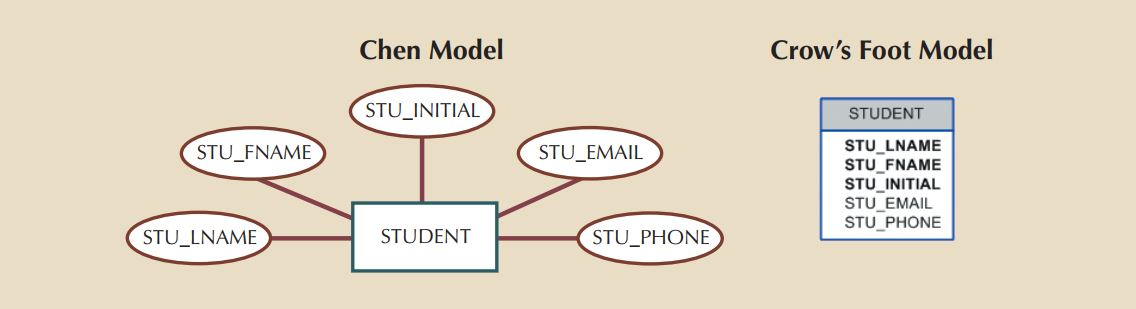
\includegraphics[scale=0.5]{Attr}
\caption{Attributes in Chen and Crow's Foot}
\end{figure}

\noindent A \textbf{required attribute} is an attribute that must have a value; in other words, it cannot be left empty. An \textbf{optional attribute} is an attribute that does not require a value; therefore, it can be left empty.\\
Attributes have a domain. A \textbf{domain} is the set of possible values for a given attribute. Attributes may share a domain. For instance, a student address and a professor
address share the same domain of all possible addresses. In fact, the data dictionary may let a newly declared attribute inherit the characteristics of an existing attribute if the
same attribute name is used. For example, the PROFESSOR and STUDENT entities may each have an attribute named ADDRESS and could therefore share a domain.\\
The ERM uses \textbf{identifiers}—one or more attributes that uniquely identify each entity instance. In the relational model, entities are mapped to tables, and the entity identifier is mapped as the table’s primary key (PK). Identifiers are underlined in the ERD. Key attributes are also underlined in a frequently used shorthand notation for the table structure, called a \textbf{relational schema}, that uses the following format:\\ \\
TABLE NAME (\uline{\textbf{{KEY\_ATTRIBUTE 1}}}, ATTRIBUTE 2, … ATTRIBUTE K)\\ \\
Ideally, an entity identifier is composed of only a single attribute. However, it is possible to use a \textbf{composite identifier}, a primary key composed of more than one attribute. The following format is used:\\ \\
TABLE NAME (\uline{\textbf{{KEY\_ATTRIBUTE 1, ATTRIBUTE 2}}}, … ATTRIBUTE K)\\ \\
Attributes are classified as simple or composite. A \textbf{composite attribute}, not to be confused with a composite key, is an attribute that can be further subdivided to yield additional attributes. For example, the attribute ADDRESS can be subdivided into street, city, state, and zip code. A \textbf{simple attribute} is an attribute that cannot be subdivided. For example, age, sex, and marital status would be classified as simple attributes.\\
A \textbf{single-valued attribute} is an attribute that can have only a single value. For example, a person can have only one Social Security number, and
a manufactured part can have only one serial number. \emph{Keep in mind that a single-valued attribute is not necessarily a simple attribute}. For instance, a part’s serial number (such as SE-08-02-189935) is single-valued, but it is a composite attribute because it can be subdivided into the region in which the part was produced (SE), the plant within that region (08), the shift within the plant (02), and the part number (189935).\\
\textbf{Multivalued attributes} are attributes that can have many values. For instance, a car’s color may be subdivided into many colors for the roof, body, and trim. In the Chen ERM, multivalued attributes are shown by a double line connecting the attribute to the entity. The Crow’s Foot notation does not identify multivalued attributes. The ERD in Figure 4.2 contains all of the components introduced thus far; note that CAR\_VIN is the primary key, and CAR\_COLOR is a multivalued attribute of the CAR entity.
\begin{figure}[H]
\centering
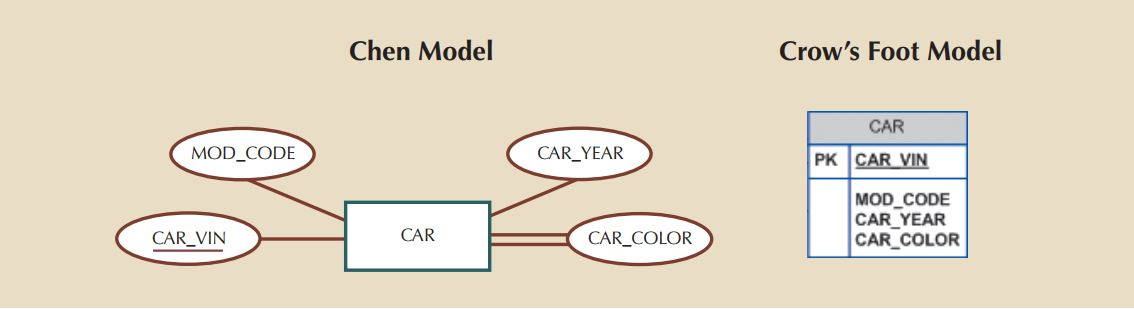
\includegraphics[scale=0.5]{Attr2}
\caption{Multivalued Attributes in an Entity}
\end{figure}
\noindent\emph{Implementing Multivalued Attributes} - Although the conceptual model can handle M:N relationships and multivalued attributes, \emph{you should not implement them in the
RDBMS}. Remember that in the relational table, each column and row intersection represents a single data value. So, if multivalued attributes exist, the designer must decide on one of two possible courses of action:
\begin{enumerate}
\item Within the original entity, create several new attributes, one for each component of the original multivalued attribute. For example, the CAR entity’s attribute CAR\_COLOR
can be split to create the new attributes CAR\_TOPCOLOR, CAR\_BODYCOLOR, and CAR\_TRIMCOLOR, which are then assigned to the CAR entity. \\
\begin{figure}[H]
\centering
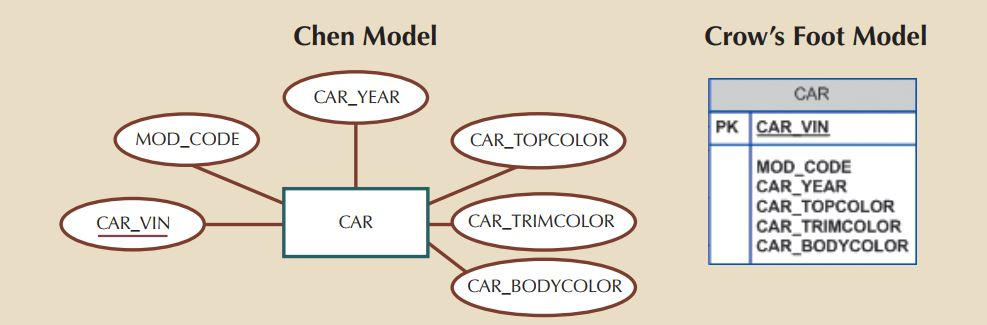
\includegraphics[scale=0.5]{Attr3}
\caption{Splitting Multivalued Attributes into New Attributes}
\end{figure}
Although this solution seems to work, its adoption can lead to major structural problems in the table. It is only acceptable if every instance will have the same number of values for the multivalued attribute, and no instance will ever have more values. However, even in this case, it is a gamble that new changes in the environment will never create a situation where an instance would have more values than before.
\item Create a new entity composed of the original multivalued attribute’s components. This new entity allows the designer to define color for different sections of the car. Then, this new CAR\_COLOR entity is related to the original CAR entity in a 1:M relationship. This is the preferred way to deal with multivalued attributes. Creating a new entity in a 1:M relationship with the original entity yields several benefits: it is a more flexible, expandable solution, and it is compatible with the relational model!
\begin{figure}[H]
\centering
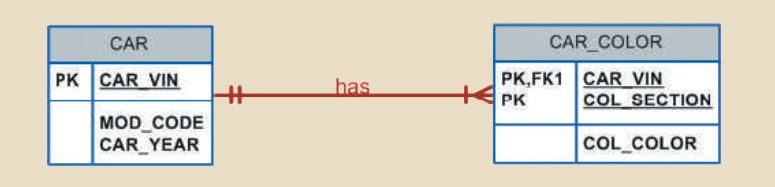
\includegraphics[scale=0.5]{Attr4}
\caption{A New Entity Set Composed of a Multivalued Attribute's Components}
\end{figure}
\end{enumerate}
\noindent Finally, a \textbf{derived attribute} is an attribute whose value is calculated (derived) from other attributes. The derived attribute need not be physically stored within the database; instead, it can be derived by using an algorithm.  A derived attribute is indicated in the Chen notation by a dashed line that connects the attribute and the entity. (See Figure 4.5.) The Crow’s Foot notation does not have a method for distinguishing the derived attribute from other attributes. Derived attributes are sometimes referred to as \emph{computed attributes}. Computing a derived attribute can be as simple as adding two attribute values located on the same row, or it can be the result of aggregating the sum of values located on many table rows (from the same table or from a different table). The decision to store derived attributes in database tables depends on the processing requirements and the constraints placed on a particular application. The designer should be able to balance the design in accordance with such constraints. 
\begin{figure}[H]
\centering
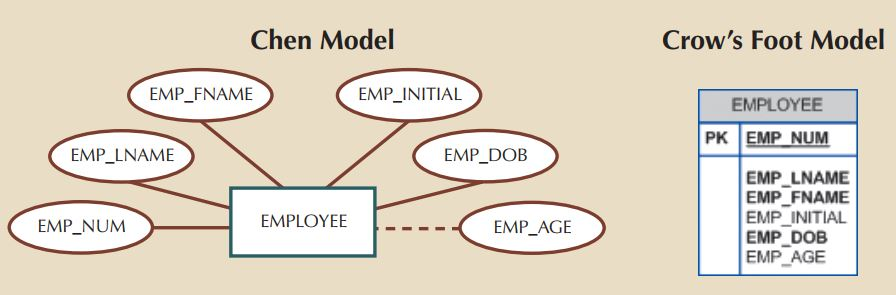
\includegraphics[scale=0.5]{Attr5}
\caption{Depiction of a Derived Attribute}
\end{figure}

%\begin{table}[H]
%\centering
%\caption{Advantages and Disadvantages of Storing Derived Attributes}
%\begin{tabular}{p{2cm} p{5cm} p{5cm}}
%\toprule
%& Stored & Not Stored \\
%\midrule
%\midrule
%Advantage & \item Saves CPU processing cycles &  \item Saves data access time\\
%& \item Saves data access time &  \item Computation always yields current value\\
%& \item Data value is readily available & \\
%& \item Can be used to keep track of historical data & \\
%
%Disadvantage & \item Requires constant maintenance to ensure derived value is current, especially if any values used in the calculation change & \item Uses CPU processing cycles\\
%& & \item Increases data access time\\
%& & \item Adds coding complexity to queries\\
%\bottomrule
%\bottomrule
%\end{tabular}
%\end{table}

\subsection{Relationships}
A relationship is an association between entities. The entities that participate in a relationship are also known as \textbf{participants}, and each relationship is identified by a name that describes the relationship. The relationship name is an active or passive verb. Relationships between entities always operate in both directions therefore both have to established.

\subsection{Connectivity and Cardinality}
The term \textbf{connectivity} is used to describe the relationship classification. \textbf{Cardinality} expresses the minimum and maximum number of entity occurrences associated with one occurrence of the related entity. \\In the ERD, cardinality is indicated by placing the appropriate numbers beside the entities, using the format (x,y). The first value represents the minimum number of associated entities, while the second value represents the maximum number of associated entities. \\Knowing the minimum and maximum number of entity occurrences is very useful at the application software level. Keep in mind that the DBMS cannot handle the implementation of the cardinalities at the table level—that capability is provided by the application software or by triggers. \\Connectivities and cardinalities are established by concise statements known as business rules. Such rules, derived from a precise and detailed description of an organization’s data environment, also establish the ERM’s entities, attributes, relationships, connectivities, cardinalities, and constraints. Because business rules define the ERM’s components, making sure that all appropriate business rules are identified is an important part of a database designer’s job.\\ The placement of the cardinalities in the ER diagram is a matter of convention. The Chen notation places the cardinalities on the side of the related entity. The Crow’s Foot and UML diagrams place the cardinalities next to the entity to which they apply.
\begin{figure}[H]
\centering
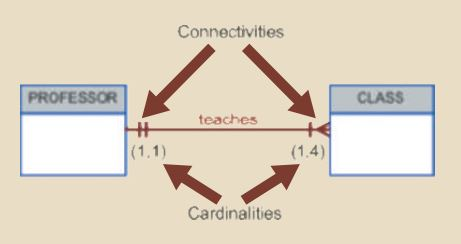
\includegraphics[scale=0.8]{ConnCard}
\caption{Connectivity and Cardinality in an ERD}
\end{figure}

\subsection{Existence Dependence}
An entity is said to be \textbf{existence-dependent} if it can exist in the database only when it is associated with another related entity occurrence. In implementation terms, an entity is existence-dependent if it has a mandatory foreign key—that is, a foreign key attribute that cannot be null. If an entity can exist apart from all of its related entities, then it is \textbf{existence-independent}, and it is referred to as a \textbf{strong entity} or \textbf{regular entity}. \\The concept of relationship strength is not part of the original ERM. Instead, this concept applies directly to Crow’s Foot diagrams. Because Crow’s Foot diagrams are used extensively to design relational databases, it is important to understand relationship strength as it affects database implementation. The Chen ERD notation is oriented toward conceptual modeling and therefore does not distinguish between weak and strong relationships.

\subsection{Relationship Strength}
The concept of relationship strength is based on how the primary key of a related entity is defined. To implement a relationship, the primary key of one entity (the parent entity,
normally on the “one” side of the 1:M relationship) appears as a foreign key in the related entity (the child entity, mostly the entity on the “many” side of the 1:M relationship). Sometimes, the foreign key also is a primary key component in the related entity.\\
A \textbf{weak relationship}, also known as a \textbf{non-identifying relationship}, exists if the primary key of the related entity does not contain a primary key component of the parent entity. By default, relationships are established by having the primary key of the parent entity appear as a foreign key (FK) on the related entity (also known as the child entity).\\ \\
A \textbf{strong (identifying) relationship} exists when the primary key of the related entity contains a primary key component of the parent entity. The Crow’s Foot notation depicts the strong (identifying) relationship with a solid line between the entities.\\
Keep in mind that the \emph{order in which the tables are created and loaded is very important}. In fact, \emph{you must load the data of the “1” side first in a 1:M relationship to avoid the possibility of referential integrity errors}, regardless of whether the relationships are weak or strong.

\subsection{Weak Entities}
In contrast to the strong or regular entity mentioned in Section 4.1.6, a weak entity is one that meets two conditions:
\begin{enumerate}
\item The entity is existence-dependent; it cannot exist without the entity with which it has a relationship.
\item The entity has a primary key that is partially or totally derived from the parent entity in the relationship.
\end{enumerate}
\begin{figure}[H]
\centering
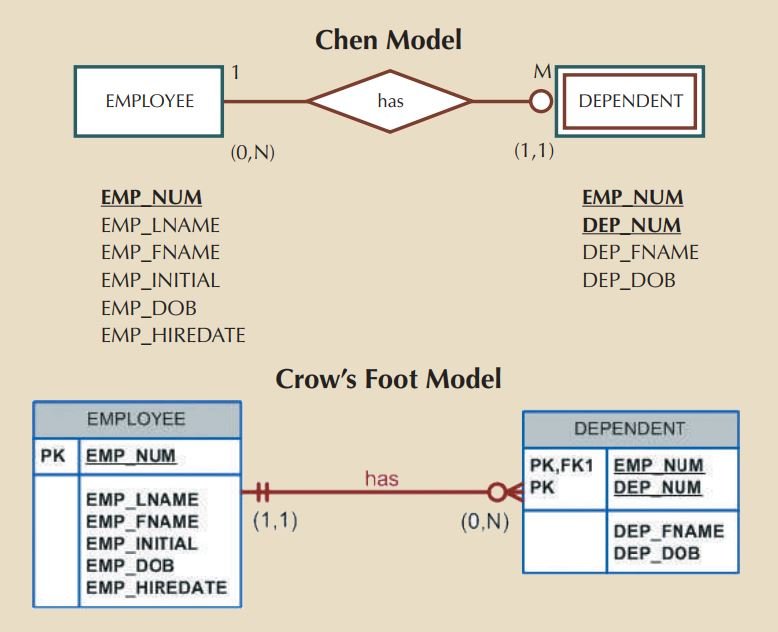
\includegraphics[scale=0.6]{Weak}
\caption{A Weak Entity in an ERD}
\end{figure}

\noindent Note that the Chen notation in Figure 4.7 identifies the weak entity by using a double-walled entity rectangle. The Crow’s Foot notation uses the relationship line and the PK/FK designation to indicate whether the related entity is weak. A strong (identifying) relationship indicates that the related entity is weak. Such a relationship means that both conditions have been met for the weak entity definition—the related entity is existence-dependent, and the PK of the related entity contains a PK component of the parent entity. Remember that the weak entity inherits part of its primary key from its strong counterpart. 

\subsection{Relationship Participation}
Participation in an entity relationship is either optional or mandatory. Recall that relationships are bidirectional; that is, they operate in both directions. Because of this nature, it is necessary to determine the connectivity of the relationship from one entity to another and back. Similarly, the specific maximum and minimum cardinalities must be determined in each direction for the relationship. Once again, you must consider the bidirectional nature of the relationship when determining participation.
\textbf{Optional participation} means that one entity occurrence does not \emph{require} a corresponding entity occurrence in a particular relationship. In Crow’s Foot notation, an optional relationship between entities is shown by drawing a small circle (O) on the side of the optional entity. The existence of an \emph{optional entity} indicates that its minimum cardinality is 0. (The term \emph{optionality} is used to label any condition in which one or more optional relationships exist.)\\
Remember that the burden of establishing the relationship is always placed on the entity that contains the foreign key. In most cases, that entity is on the “many” side of the relationship.\\ \\
\textbf{Mandatory participation} means that one entity occurrence requires a corresponding entity occurrence in a particular relationship. If no optionality symbol is depicted
with the entity, the entity is assumed to exist in a mandatory relationship with the related entity. If the mandatory participation is depicted graphically, it is typically shown as a small hash mark across the relationship line, similar to the Crow’s Foot depiction of a connectivity of 1. The existence of a mandatory relationship indicates that the minimum
cardinality is at least 1 for the mandatory entity.\\ \\
You might be tempted to conclude that relationships are weak when they occur between entities in an optional relationship and that relationships are strong when they occur between entities in a mandatory relationship. However, this conclusion is not warranted. Keep in mind that relationship participation and relationship strength do not describe the same thing. You are likely to encounter a strong relationship when one entity is optional to another. Also, it is just as possible for a weak relationship to be established when one entity is mandatory to another. The relationship strength depends on how the PK of the related entity is formulated, while the relationship participation depends on how the business rule is written. Failure to understand this distinction may lead to poor design decisions that cause major problems when table rows are inserted or deleted.\\\\
It is important that you clearly understand the distinction between mandatory and optional participation in relationships. Otherwise, you might develop designs in which
awkward and unnecessary temporary rows (entity instances) must be created just to accommodate the creation of required entities.

\subsection{Relationship Degree}
A \textbf{relationship degree} indicates the number of entities or participants associated with a relationship. A \textbf{unary relationship} exists when an association is maintained within a single entity. Such a relationship is known as a \textbf{recursive relationship}. A \textbf{binary relationship} exists when two entities are associated. A \textbf{ternary relationship} exists when three entities are associated. Although higher degrees exist, they are rare and are not specifically named. (For example, an association of four entities is described simply as a \emph{four-degree relationship}.) Figure 4.8 shows these types of relationship degrees.
\begin{figure}[H]
\centering
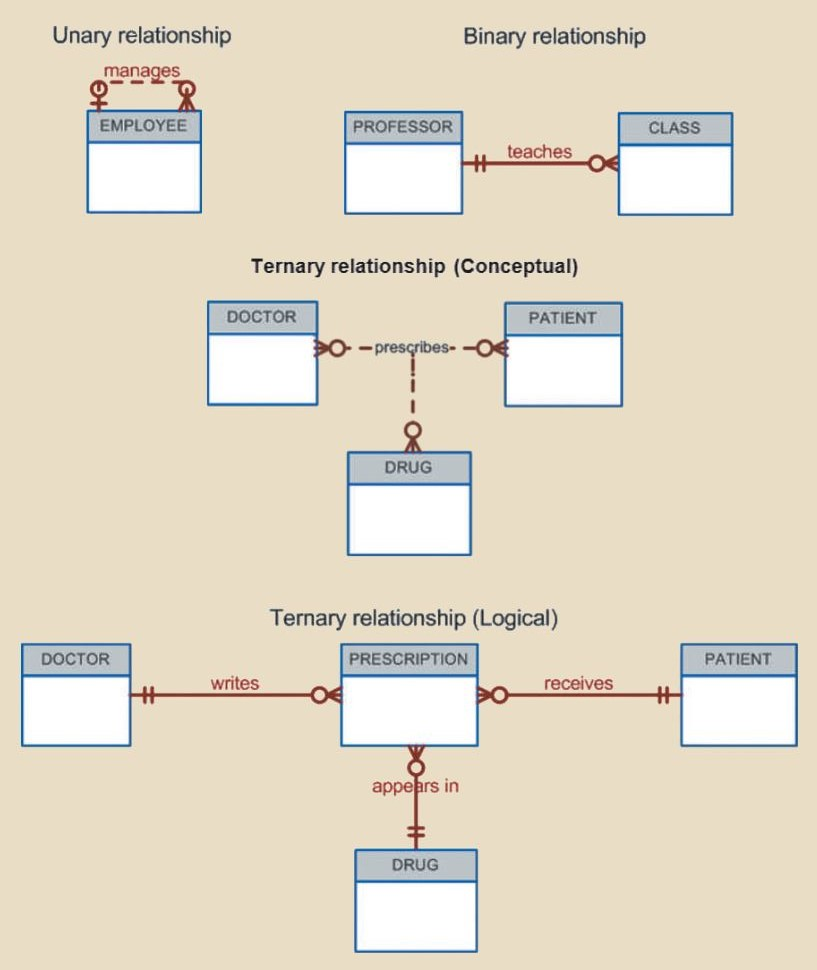
\includegraphics[scale=0.6]{Relation}
\caption{Three types of Relationship Degree}
\end{figure}

\subsection{Recursive Relationships}
As you just learned, a \emph{recursive relationship} is one in which a relationship can exist between occurrences of the same entity set. (Naturally, such a condition is found within a unary relationship.) For example, a 1:M unary relationship can be expressed by “an EMPLOYEE may manage many EMPLOYEEs, and each EMPLOYEE is managed by one EMPLOYEE.” Also, as long as polygamy is not legal, a 1:1 unary relationship may be expressed by “an EMPLOYEE may be married to one and only one other EMPLOYEE.” Finally, the M:N unary relationship may be expressed by “a COURSE may be a prerequisite to many other COURSEs, and each COURSE may have many other COURSEs as prerequisites.” Those relationships are shown in Figure 4.9.
\begin{figure}[H]
\centering
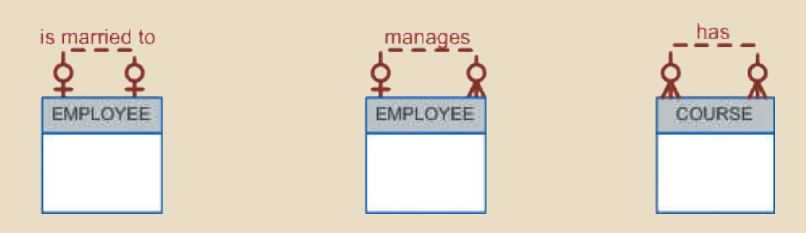
\includegraphics[scale=0.6]{Recur}
\caption{An ER Representation of Recursive Relationships}
\end{figure}
\noindent One common pitfall when working with unary relationships is to confuse participation with referential integrity. In theory, participation and referential integrity are very different concepts and are normally easy to distinguish in binary relationships. In practical terms, conversely, participation and referential integrity are very similar because they are both implemented through constraints on the same set of attributes. This similarity often leads to confusion when the concepts are applied within the limited structure of a unary relationship. Referential integrity deals with the correspondence of values in the foreign key with values in the related primary key. Referential integrity is not bidirectional. In practical terms, both participation and referential integrity involve the values used as primary keys and foreign keys to implement the relationship. Referential integrity requires that the values in the foreign key correspond to values in the primary key. In one direction, participation considers whether the foreign key can contain a null. In the other direction, participation considers whether every value in the primary key must appear as a value in the foreign key. 

\subsection{Associative (Composite) Entities}
M:N relationships are a valid construct at the conceptual level, and therefore are found frequently during the ER modeling process. However, implementing the M:N
relationship, particularly in the relational model, requires the use of an additional entity. The ER model uses the associative entity to represent an M:N relationship between two or more entities. This associative entity, also called a \emph{composite} or \emph{bridge entity}, is in a 1:M relationship with the parent entities and is composed of
the primary key attributes of each parent entity. Furthermore, the associative entity can have additional attributes of its own. When using the Crow’s Foot notation, the associative entity is identified as a strong (identifying) relationship, as indicated by the solid relationship lines between the parents and the associative entity.

\section{Developing an ER diagram}
The process of database design is iterative rather than a linear or sequential process. The verb iterate means “to do again or repeatedly.” Thus, an \textbf{iterative process} is based on repetition of processes and procedures. Building an ERD usually involves the following activities:
\begin{itemize}
\item Create a detailed narrative of the organization’s description of operations.
\item Identify the business rules based on the description of operations.
\item Identify the main entities and relationships from the business rules.
\item Develop the initial ERD.
\item Identify the attributes and primary keys that adequately describe the entities.
\item Revise and review the ERD.
\end{itemize}
During the review process, additional objects, attributes, and relationships probably will be uncovered. Therefore, the basic ERM will be modified to incorporate the newly
discovered ER components. Subsequently, another round of reviews might yield additional components or clarification of the existing diagram. The process is repeated until
the end users and designers agree that the ERD is a fair representation of the organization’s activities and functions. During the design process, the database designer does not depend simply on interviews to help define entities, attributes, and relationships. A surprising amount of information can be gathered by examining the business forms and reports that an organization uses in its daily operations.
\begin{figure}[H]
\centering
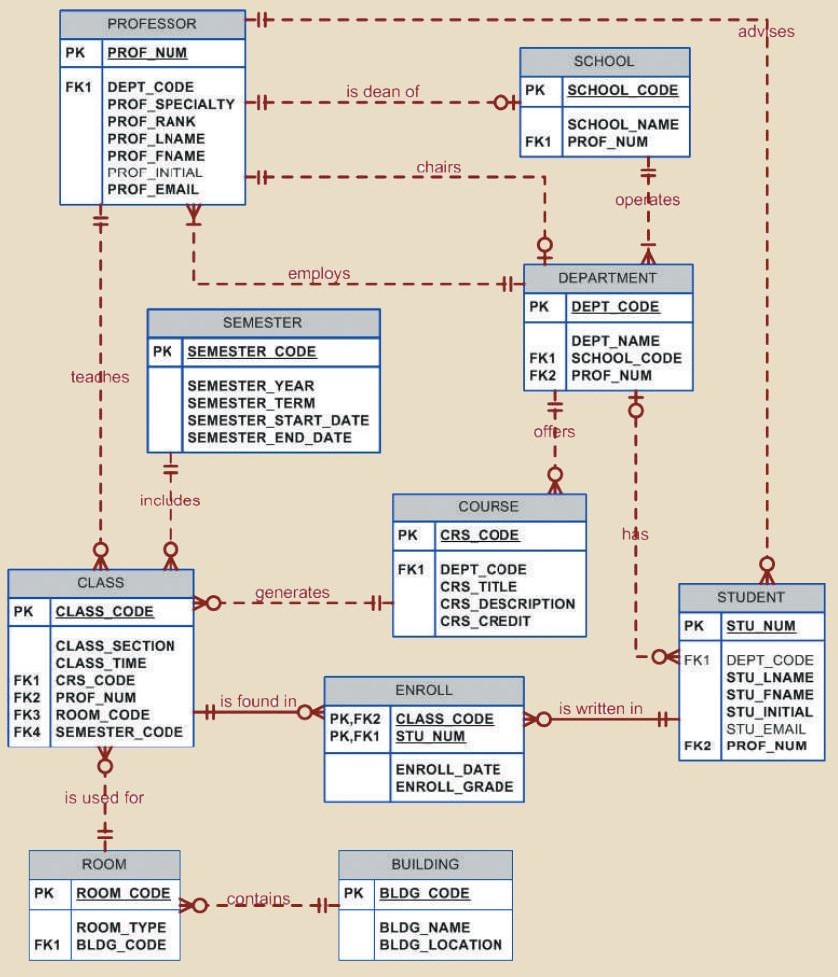
\includegraphics[scale=0.6]{ERDComp}
\caption{An Example of a Complete ERD}
\end{figure}

\noindent Although we focus on Crow’s Foot notation to develop the diagram above, as mentioned at the beginning of this unit, UML notation is also popular for conceptual and
implementation modeling. Figure 4.11 shows the conceptual UML class diagram for same ERD above. If you are a good observer, you will also notice that the UML class diagrams in Figures 4.11 and 4.12 show the entity and attribute names but do not identify the primary key attributes. The reason goes back to UML’s roots. UML class diagrams are an object-oriented modeling language, and therefore do not support the notion of “primary or foreign keys” found mainly in the relational world. Rather, in the object-oriented world, objects inherit a unique object identifier at creation time.

\begin{figure}[H]
\centering
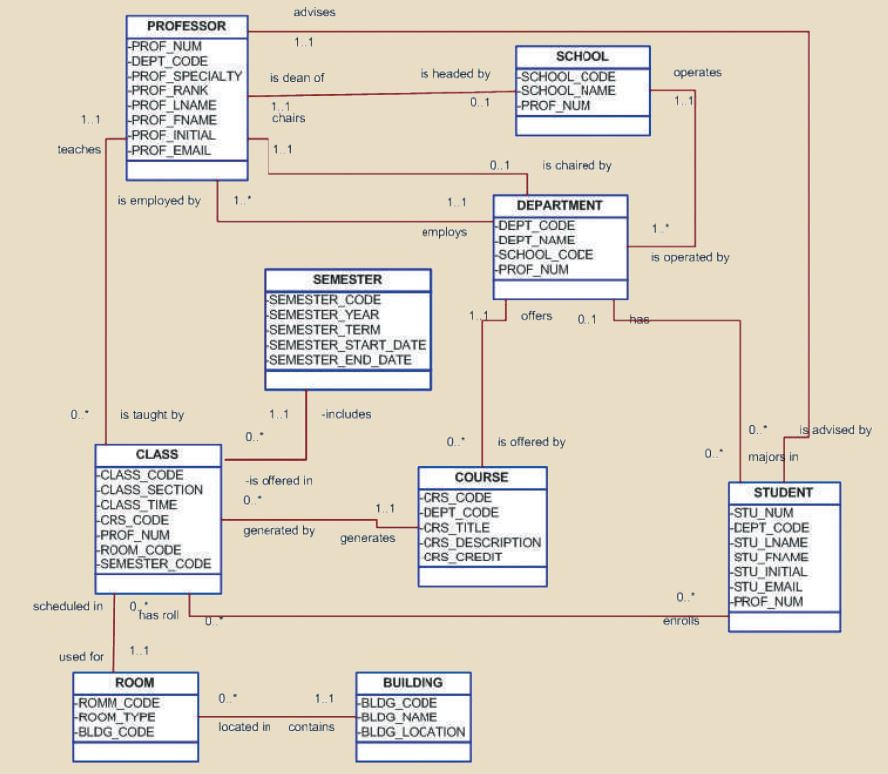
\includegraphics[scale=0.7]{UML1}
\caption{A Conceptual UML Class Diagram}
\end{figure}
\begin{figure}[H]
\centering
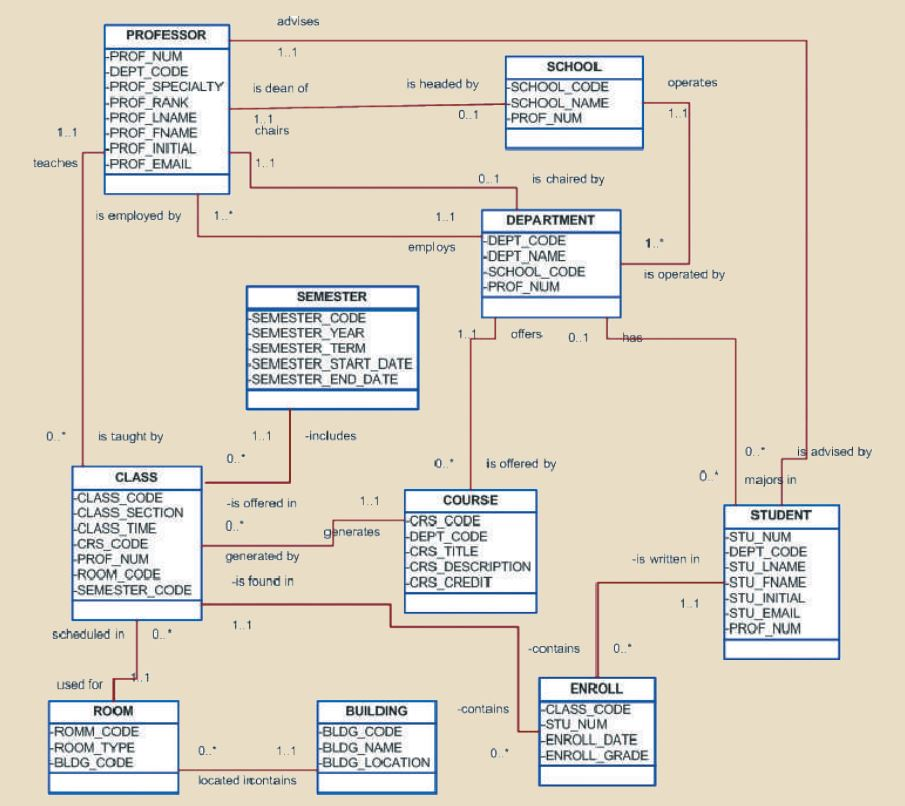
\includegraphics[scale=0.7]{UML2}
\caption{An Implementation-ready UML Class Diagram}
\end{figure}

\section{Database Design Challenges: Conflicting Goals}
Database designers must often make design compromises that are triggered by conflicting goals, such as adherence to design standards (design elegance), processing speed,
and information requirements.
\begin{itemize}
\item \emph{Design standards}. The database design must conform to design standards. Such standards guide you in developing logical structures that minimize data redundancies,
thereby minimizing the likelihood that destructive data anomalies will occur. Without design standards, it is nearly impossible to formulate a proper design process, to evaluate an existing design, or to trace the likely logical impact of changes in design.
\item \emph{Processing speed}. In many organizations, particularly those that generate large numbers of transactions, high processing speeds are often a top priority in database
design. High processing speed means minimal access time, which may be achieved by minimizing the number and complexity of logically desirable relationships.
\item \emph{Information requirements}. The quest for timely information might be the focus of database design. Complex information requirements may dictate data transformations, and they may expand the number of entities and attributes within the design. Therefore, the database may have to sacrifice some of its “clean” design structures and
high transaction speed to ensure maximum information generation.
\end{itemize}

\noindent A design that meets all logical requirements and design conventions is an important goal. However, if this perfect design fails to meet the customer’s transaction speed and information requirements, the designer will not have done a proper job from the end user’s point of view. Compromises are a fact of life in the real world of database design.
Even while focusing on the entities, attributes, relationships, and constraints, the designer should begin thinking about end-user requirements such as performance, security, shared access, and data integrity. The designer must consider processing requirements and verify that all update, retrieval, and deletion options are available.\\
Finally, a design is of little value unless the end product can deliver all specified query and reporting requirements. You will probably discover that even the best design process produces an ERD that requires further changes mandated by operational requirements. Such changes should not discourage you from using the process. ER modeling is essential in the development of a sound design that can meet the demands of adjustment and growth. Using ERDs yields perhaps the richest bonus of all: a thorough understanding of how an organization really functions. Occasionally, design and implementation problems do not yield “clean” implementation solutions.\\\\
Your job as a database designer is to use your professional judgment to yield a solution that meets the requirements imposed by business rules, processing requirements, and basic design principles.\\\\
Finally, document, document, and document! Put all design activities in writing, and then review what you have written. Documentation not only helps you stay on track
during the design process, it also enables you and your coworkers to pick up the design thread when the time comes to modify the design. Although the need for documentation should be obvious, one of the most vexing problems in database and systems analysis work is that this need is often ignored in the design and implementation stages. The development of organizational documentation standards is an important aspect of ensuring data compatibility and coherence.

\section{The Extended Entity Relationship Model}
\subsection{Entity Supertypes and Subtypes}
\subsection{Specialization Hierarchy}
\subsection{Inheritance}
\subsection{Subtype Discriminator}
\subsection{Disjoint and Overlapping Constraints}
\subsection{Specialization and Generalization}

\section{Entity Clustering}
\section{Entity Integrity}
\subsection{Natural Keys and Primary Keys}
\subsection{Primary Key Guidelines}
\subsection{When to Use Composite Primary Keys}
\subsection{When to Use Surrogate Primary Keys}

\section{Design Cases}
\subsection{Implementing 1:1 Relationships}
\subsection{Maintaining History of Time-Variant Data}
\subsection{Fan Traps}
\subsection{Redundant Relationships}

\pagebreak
\tikzset{
    zig zag to/.style={
        to path={(\tikztostart) -| ($(\tikztostart)!#1!(\tikztotarget)$) |- (\tikztotarget) \tikztonodes}
    },
    zig zag to/.default=0.5,
    one to one/.style={
        one-one, zig zag to
    },    
    one to none/.style={
        one-, zig zag to
    },    
    oone to none/.style={
        oone-, zig zag to
    },    
    omany to none/.style={
        omany-, zig zag to
    },    
    one to many/.style={
        one-crow's foot, zig zag to,
    },
    one to omany/.style={
        one-omany, zig zag to
    },      
    many to one/.style={
        crow's foot-one, zig zag to
    },
    many to many/.style={
        crow's foot-crow's foot, zig zag to
    }, 
    many to none/.style={ 
        crow's foot-, zig zag to 
    },
}    
\makeatletter
\pgfarrowsdeclare{crow's foot}{crow's foot}
{
    \pgfarrowsleftextend{+-.5\pgflinewidth}%
    \pgfarrowsrightextend{+.5\pgflinewidth}%
}
{
    \pgfutil@tempdima=0.6pt%
    %\advance\pgfutil@tempdima by.25\pgflinewidth%
    \pgfsetdash{}{+0pt}%
    \pgfsetmiterjoin%
    \pgfpathmoveto{\pgfqpoint{0pt}{-9\pgfutil@tempdima}}%
    \pgfpathlineto{\pgfqpoint{-13\pgfutil@tempdima}{0pt}}%
    \pgfpathlineto{\pgfqpoint{0pt}{9\pgfutil@tempdima}}%
    \pgfpathmoveto{\pgfqpoint{0\pgfutil@tempdima}{0\pgfutil@tempdima}}%
    \pgfpathmoveto{\pgfqpoint{-8pt}{-6pt}}% 
    \pgfpathlineto{\pgfqpoint{-8pt}{-6pt}}%  
    \pgfpathlineto{\pgfqpoint{-8pt}{6pt}}% 
    \pgfusepathqstroke%
}

\pgfarrowsdeclare{omany}{omany}
{
    \pgfarrowsleftextend{+-.5\pgflinewidth}%
    \pgfarrowsrightextend{+.5\pgflinewidth}%
}
{
    \pgfutil@tempdima=0.6pt%
    %\advance\pgfutil@tempdima by.25\pgflinewidth%
    \pgfsetdash{}{+0pt}%
    \pgfsetmiterjoin%
    \pgfpathmoveto{\pgfqpoint{0pt}{-9\pgfutil@tempdima}}%
    \pgfpathlineto{\pgfqpoint{-13\pgfutil@tempdima}{0pt}}%
    \pgfpathlineto{\pgfqpoint{0pt}{9\pgfutil@tempdima}}%
    \pgfpathmoveto{\pgfqpoint{0\pgfutil@tempdima}{0\pgfutil@tempdima}}%  
    \pgfpathmoveto{\pgfqpoint{0\pgfutil@tempdima}{0\pgfutil@tempdima}}%
    \pgfpathmoveto{\pgfqpoint{-6pt}{-6pt}}% 
    \pgfpathcircle{\pgfpoint{-11.5pt}{0}} {3.5pt}
    \pgfusepathqstroke%
}

\pgfarrowsdeclare{oone}{oone}
{
    \pgfarrowsleftextend{+-.5\pgflinewidth}%
    \pgfarrowsrightextend{+.5\pgflinewidth}%
}
{
    \pgfutil@tempdima=0.6pt%
    %\advance\pgfutil@tempdima by.25\pgflinewidth%
    \pgfsetdash{}{+0pt}%
    \pgfsetmiterjoin%
     \pgfpathmoveto{\pgfqpoint{0\pgfutil@tempdima}{0\pgfutil@tempdima}}%
    \pgfpathmoveto{\pgfqpoint{-6pt}{-6pt}}% 
    \pgfpathlineto{\pgfqpoint{-6pt}{-6pt}}%  
    \pgfpathlineto{\pgfqpoint{-6pt}{6pt}}% 
    \pgfpathcircle{\pgfpoint{-11.5pt}{0}} {3.5pt}
    \pgfusepathqstroke%
}

\pgfarrowsdeclare{one}{one}
{
    \pgfarrowsleftextend{+-.5\pgflinewidth}%
    \pgfarrowsrightextend{+.5\pgflinewidth}%
}
{
    \pgfutil@tempdima=0.6pt%
    %\advance\pgfutil@tempdima by.25\pgflinewidth%
    \pgfsetdash{}{+0pt}%
    \pgfsetmiterjoin%
    \pgfpathmoveto{\pgfqpoint{0\pgfutil@tempdima}{0\pgfutil@tempdima}}%
    \pgfpathmoveto{\pgfqpoint{-6pt}{-6pt}}% 
    \pgfpathlineto{\pgfqpoint{-6pt}{-6pt}}%  
    \pgfpathlineto{\pgfqpoint{-6pt}{6pt}}% 
    \pgfpathmoveto{\pgfqpoint{0\pgfutil@tempdima}{0\pgfutil@tempdima}}%
    \pgfpathmoveto{\pgfqpoint{-8pt}{-6pt}}% 
    \pgfpathlineto{\pgfqpoint{-8pt}{-6pt}}%  
    \pgfpathlineto{\pgfqpoint{-8pt}{6pt}}%    
    \pgfusepathqstroke%
}

\section{Notation Versions}  
\begin{tabular}{lcc}
    \toprule
    \toprule
    Notation & IEM & CHEN \\
    \midrule
    \midrule
    one to none &
        \tikz{\draw[one to none] (0,0) -- ++(1.5,0);} & 1:0\\
    one to one & \tikz{\draw[one to one] (0,0) -- ++(1.5,0);} & 1:1\\
    one to many & \tikz{\draw[one to many] (0,0) -- ++(1.5,0);} & 1:N\\
    many to none & \tikz{\draw[many to none] (0,0) -- ++(1.5,0);} & N:0\\
    one to (none or one or many) &\tikz{\draw[one to omany] (0,0) -- ++(1.5,0);} & \\ 
    many to one & \tikz{\draw[many to one] (0,0) -- ++(1.5,0);} & N:1\\ 
    many to many &\tikz{\draw[many to many] (0,0) -- ++(1.5,0);} & N:M\\
    (none or one or many) to none &\tikz{\draw[omany to none] (0,0) -- ++(1.5,0);} & \\
    (none or one) to none &\tikz{\draw[oone to none] (0,0) -- ++(1.5,0);} & \\
    \bottomrule
\end{tabular}
\end{document}